% \documentclass{article}
% \usepackage{amsmath}
% \usepackage{amsthm}
% \usepackage{enumerate}
% \usepackage{bookmark}
% \usepackage{graphicx}
% \usepackage{multirow}
% \usepackage{adjustbox}
% \usepackage{wrapfig}
% \usepackage{subcaption}
% \usepackage{color}
% \usepackage[dvipsnames]{xcolor}

% \usepackage{amssymb,amsmath,amsthm,amsfonts}
% \usepackage{mathrsfs}
% \usepackage{dsfont}
% \usepackage{enumerate}

% \usepackage{amssymb,amsmath,amsthm,amsfonts}
\usepackage{mathrsfs}
\usepackage{dsfont}
\usepackage{enumerate}

%\newtheorem{mdef}{Definition}
%\newtheorem{theorem}{Theorem}
\newcommand{\eqsplit}[2]{
  \begin{equation}\label{#2}
    \begin{split}
      #1
    \end{split}
  \end{equation}}
\newcommand{\eqnsplit}[1]{
  \begin{eqnarray*}
    #1
  \end{eqnarray*}}
\newcommand{\tran}[1]{
  \tilde{#1}
}
\newcommand{\td}[2]{
  \frac{d #1}{d #2}
}
\newcommand{\pd}[2]{
  \frac{\partial #1}{\partial #2}
}
\newcommand{\ppd}[2]{
  \frac{\partial^2 #1}{\partial #2^2}
}
\newcommand{\pdd}[3]{
  \frac{\partial^2 #1}{\partial #2 \partial #3}
}
\newcommand{\otd}[1]{
  \frac{d}{d #1}
}
\newcommand{\opd}[1]{
  \frac{\partial}{\partial #1}
}
\newcommand{\oppd}[1]{
  \frac{\partial^2}{\partial #1^2}
}
\newcommand{\opdd}[2]{
  \frac{\partial^2}{\partial #1 \partial #2}
}
\newcommand{\ket}[1]{
  |#1\rangle
}
\newcommand{\bra}[1]{
  \langle#1|
}
\newcommand{\inn}[1]{
  \langle#1\rangle
}
\newcommand{\mean}[1]{
  \langle#1\rangle
}
\newcommand{\tr}{
  \text{tr}\,
}
\newcommand{\re}{
  \text{Re}\,
}
\newcommand\im{
  \text{Im}\,
}
\newcommand{\var}{
  \text{var}
}
\newcommand{\arcsinh}{
  \sinh^{-1}
}
\newcommand{\arccosh}{
  \cosh^{-1}
}
\newcommand{\erfc}{
  \text{erfc}
}
\newcommand{\E}{
  \mathbb{E}
}
\renewcommand{\P}{
  \mathbb{P}
}
\newcommand{\I}[1]{
  \mathbf{1}_{\{#1\}}
}
\newcommand{\1}[1]{
  \mathds{1}_{\{#1\}}
}
\newcommand{\diag}{
  \text{diag\,}
}
\newcommand{\M}{
  {\text{max}}
}
\newcommand{\m}{
  {\text{min}}
}
\newcommand{\ph}{
  {\text{arg}\,}
}
\newcommand\erf{
  \text{erf}
}
\renewcommand\vec[1]{
  \mathbf{#1}
}
\newcommand\mtx[1]{
  \mathbf{#1}
}
\newcommand\ed{
  \,{\buildrel d \over =}\,
}





\documentclass[11pt,a4]{amsart}
%\usepackage{amsmath}
%\usepackage{amsthm}
%\usepackage{enumerate}
\usepackage[bookmarks=true]{hyperref}
%\usepackage{bookmark}
\usepackage{graphicx}
%\usepackage{multirow}
%\usepackage{adjustbox}
%\usepackage{wrapfig}
%\usepackage{subcaption}
\usepackage{color}
\usepackage[dvipsnames]{xcolor}

\usepackage{amssymb,amsmath,amsthm,amsfonts}
%\usepackage{mathrsfs}
%\usepackage{dsfont}
%\usepackage{enumerate}

%\usepackage{amssymb,amsmath,amsthm,amsfonts}
\usepackage{mathrsfs}
\usepackage{dsfont}
\usepackage{enumerate}

%\newtheorem{mdef}{Definition}
%\newtheorem{theorem}{Theorem}
\newcommand{\eqsplit}[2]{
  \begin{equation}\label{#2}
    \begin{split}
      #1
    \end{split}
  \end{equation}}
\newcommand{\eqnsplit}[1]{
  \begin{eqnarray*}
    #1
  \end{eqnarray*}}
\newcommand{\tran}[1]{
  \tilde{#1}
}
\newcommand{\td}[2]{
  \frac{d #1}{d #2}
}
\newcommand{\pd}[2]{
  \frac{\partial #1}{\partial #2}
}
\newcommand{\ppd}[2]{
  \frac{\partial^2 #1}{\partial #2^2}
}
\newcommand{\pdd}[3]{
  \frac{\partial^2 #1}{\partial #2 \partial #3}
}
\newcommand{\otd}[1]{
  \frac{d}{d #1}
}
\newcommand{\opd}[1]{
  \frac{\partial}{\partial #1}
}
\newcommand{\oppd}[1]{
  \frac{\partial^2}{\partial #1^2}
}
\newcommand{\opdd}[2]{
  \frac{\partial^2}{\partial #1 \partial #2}
}
\newcommand{\ket}[1]{
  |#1\rangle
}
\newcommand{\bra}[1]{
  \langle#1|
}
\newcommand{\inn}[1]{
  \langle#1\rangle
}
\newcommand{\mean}[1]{
  \langle#1\rangle
}
\newcommand{\tr}{
  \text{tr}\,
}
\newcommand{\re}{
  \text{Re}\,
}
\newcommand\im{
  \text{Im}\,
}
\newcommand{\var}{
  \text{var}
}
\newcommand{\arcsinh}{
  \sinh^{-1}
}
\newcommand{\arccosh}{
  \cosh^{-1}
}
\newcommand{\erfc}{
  \text{erfc}
}
\newcommand{\E}{
  \mathbb{E}
}
\renewcommand{\P}{
  \mathbb{P}
}
\newcommand{\I}[1]{
  \mathbf{1}_{\{#1\}}
}
\newcommand{\1}[1]{
  \mathds{1}_{\{#1\}}
}
\newcommand{\diag}{
  \text{diag\,}
}
\newcommand{\M}{
  {\text{max}}
}
\newcommand{\m}{
  {\text{min}}
}
\newcommand{\ph}{
  {\text{arg}\,}
}
\newcommand\erf{
  \text{erf}
}
\renewcommand\vec[1]{
  \mathbf{#1}
}
\newcommand\mtx[1]{
  \mathbf{#1}
}
\newcommand\ed{
  \,{\buildrel d \over =}\,
}



%\usepackage{amssymb,amsmath,amsthm,amsfonts}
\usepackage{mathrsfs}
\usepackage{dsfont}
\usepackage{enumerate}

%\newtheorem{mdef}{Definition}
%\newtheorem{theorem}{Theorem}
\newcommand{\eqsplit}[2]{
  \begin{equation}\label{#2}
    \begin{split}
      #1
    \end{split}
  \end{equation}}
\newcommand{\eqnsplit}[1]{
  \begin{eqnarray*}
    #1
  \end{eqnarray*}}
\newcommand{\tran}[1]{
  \tilde{#1}
}
\newcommand{\td}[2]{
  \frac{d #1}{d #2}
}
\newcommand{\pd}[2]{
  \frac{\partial #1}{\partial #2}
}
\newcommand{\ppd}[2]{
  \frac{\partial^2 #1}{\partial #2^2}
}
\newcommand{\pdd}[3]{
  \frac{\partial^2 #1}{\partial #2 \partial #3}
}
\newcommand{\otd}[1]{
  \frac{d}{d #1}
}
\newcommand{\opd}[1]{
  \frac{\partial}{\partial #1}
}
\newcommand{\oppd}[1]{
  \frac{\partial^2}{\partial #1^2}
}
\newcommand{\opdd}[2]{
  \frac{\partial^2}{\partial #1 \partial #2}
}
\newcommand{\ket}[1]{
  |#1\rangle
}
\newcommand{\bra}[1]{
  \langle#1|
}
\newcommand{\inn}[1]{
  \langle#1\rangle
}
\newcommand{\mean}[1]{
  \langle#1\rangle
}
\newcommand{\tr}{
  \text{tr}\,
}
\newcommand{\re}{
  \text{Re}\,
}
\newcommand\im{
  \text{Im}\,
}
\newcommand{\var}{
  \text{var}
}
\newcommand{\arcsinh}{
  \sinh^{-1}
}
\newcommand{\arccosh}{
  \cosh^{-1}
}
\newcommand{\erfc}{
  \text{erfc}
}
\newcommand{\E}{
  \mathbb{E}
}
\renewcommand{\P}{
  \mathbb{P}
}
\newcommand{\I}[1]{
  \mathbf{1}_{\{#1\}}
}
\newcommand{\1}[1]{
  \mathds{1}_{\{#1\}}
}
\newcommand{\diag}{
  \text{diag\,}
}
\newcommand{\M}{
  {\text{max}}
}
\newcommand{\m}{
  {\text{min}}
}
\newcommand{\ph}{
  {\text{arg}\,}
}
\newcommand\erf{
  \text{erf}
}
\renewcommand\vec[1]{
  \mathbf{#1}
}
\newcommand\mtx[1]{
  \mathbf{#1}
}
\newcommand\ed{
  \,{\buildrel d \over =}\,
}




\textwidth 6.50in
\topmargin -0.50in
\oddsidemargin 0in
\evensidemargin 0in
\textheight 9.00in
%\pagestyle{plain}
\definecolor{darkblue}{rgb}{.2, 0.2,.8}
\definecolor{darkgreen}{rgb}{0,0.5,0.3}
\definecolor{darkred}{rgb}{.8, .1,.1}
\newcommand{\pd}{\partial}
\newcommand{\red}{\color{darkred}}
\newcommand{\blue}{\color{darkblue}}
\newcommand{\green}{\color{darkgreen}}
\newcommand{\black}{\color{black}}
\newcommand{\levy}{L\'evy}
\newcommand{\slln}{strong law of large numbers}
\newcommand{\clt}{central limit theorem}
\newcommand{\sde}{stochastic \de}
\newcommand{\de}{differential equation}
\newcommand{\mregvar}{multivariate \regvar}
\newcommand{\garch}{{\rm GARCH}$(1,1)$}
\newcommand{\spr}{stochastic process}
\newcommand{\It}{It\^o}
\newcommand{\sta}{St\u aric\u a}
\newcommand{\ex}{{\rm e}\,}
\newcommand{\sas}{s$\alpha$s}
\newcommand{\civ}{\stackrel{v}{\rightarrow}}
\newcommand{\asy}{asymptotic}
\newcommand {\hatt} {\hat{\theta}}
\newcommand {\hattg} {\hat{\theta}_{MLE}}
\newcommand {\hattz} {\hat{\theta}_0}
\newcommand {\hatb} {\hat{\beta}}
\newcommand {\hatbg} {\hat{\beta}_G}
\newcommand {\spp} {^\prime}
\newcommand{\ts}{time series}
\newcommand{\tsa}{\ts\ analysis}
\newcommand{\garchpq}{{\rm GARCH}$(p,q)$}
\def\theequation{\thesection.\arabic{equation}}
\def\tag{\refstepcounter{equation}\leqno }
\def\neqno{\refstepcounter{equation}\leqno(\thesection.\arabic{equation})}
\newtheorem{lemma}{Lemma}[section]
\newtheorem{figur}[lemma]{Figure}
\newtheorem{theorem}[lemma]{Theorem}
\newcommand{\Leb}{{\mathbb L}{\mathbb E}{\mathbb B}}
\newcommand{\bbc}{{\mathbb C}}
\newtheorem{proposition}[lemma]{Proposition}
\newtheorem{definition}[lemma]{Definition}
\newtheorem{corollary}[lemma]{Corollary}
\newtheorem{example}[lemma]{Example}
\newtheorem{exercise}[lemma]{Exercise}
\newtheorem{remark}[lemma]{Remark}
\newtheorem{fig}[lemma]{Figure}
\newtheorem{tab}[lemma]{Table}
\newtheorem{hypothesis}{Hypothesis}
\newcommand{\play}{\displaystyle}
\newcommand{\rmk}{\noindent R{\sc emark}}
\newcommand{\cid}{\stackrel{d}{\rightarrow}}
\newcommand{\cip}{\stackrel{P}{\rightarrow}}
\newcommand{\reference}{\hangindent=5pc\hangafter=1}
\newcommand{\MC}{Markov chain}
\newcommand{\bfQ}{{\bf Q}}
\newcommand{\bfM}{{\bf M}}
\newcommand{\bfu}{{\bf u}}
\newcommand{\bfv}{{\bf v}}
\newcommand{\bfV}{{\bf V}}
\newcommand{\bfU}{{\bf U}}
\newcommand{\bfR}{{\bf R}}
\newcommand{\bfC}{{\bf C}}
\newcommand{\bfF}{{\bf F}}
\newcommand{\RV}{{\rm RV}}
\newcommand{\LN}{{\rm LN}}
\newcommand{\WE}{{\rm WE}}
\newcommand{\bth}{\begin{theorem}}
\newcommand{\ethe}{\end{theorem}}
\newcommand{\sv}{stochastic volatility}
\newcommand{\bre}{\begin{remark}\em }
\newcommand{\ere}{\end{remark}}
\newcommand{\fre}{frequenc}
\newcommand{\ble}{\begin{lemma}}
\newcommand{\ele}{\end{lemma}}
\newcommand{\sre}{stochastic recurrence equation}
\newcommand{\pp}{point process}
\newcommand{\bde}{\begin{definition}}
\newcommand{\ede}{\end{definition}}
\newcommand{\bco}{\begin{corollary}}
\newcommand{\eco}{\end{corollary}}

\newcommand{\bpr}{\begin{proposition}}
\newcommand{\epr}{\end{proposition}}

\newcommand{\bexer}{\begin{exercise}}
\newcommand{\eexer}{\end{exercise}}

\newcommand{\bexam}{\begin{example}}
\newcommand{\eexam}{\end{example}}

\newcommand{\bfi}{\begin{fig}}
\newcommand{\efi}{\end{fig}}

\newcommand{\btab}{\begin{tab}}
\newcommand{\etab}{\end{tab}}
%\renewcommand{\thetab}{\arabic{section}.9.\arabic{tab}}

\newcommand{\edf}{empirical distribution function}
\newcommand{\epro}{empirical process}
\newcommand{\per}{periodogram}
\newcommand{\pf}{{\bf Proof.}}
\newcommand{\lhs}{left-hand side}
\newcommand{\fidi}{finite-dimensional distribution}
\newcommand{\rv}{random variable}
\newcommand{\DA}{{\rm DA}}
\newcommand{\DNA}{{\rm DNA}}
\newcommand{\MDA}{{\rm MDA}}
\newcommand{\sign}{{\rm sign}}
\newcommand{\PRM}{{\rm PRM}}
\newcommand{\card}{{\rm card}}
\newcommand{\var}{{\rm var}}
\newcommand{\med}{{\rm med}}
\newcommand{\cov}{{\rm cov}}
\newcommand{\corr}{{\rm corr}}
\newcommand{\as}{{\rm a.s.}}
\newcommand{\io}{{\rm i.o.}}
\newcommand{\Pois}{\rm Poisson}

\newcommand{\bfth}{\mbox{\boldmath$\theta$}}
\newcommand{\bfTh}{\mbox{\boldmath$\Theta$}}
\newcommand{\bfmu}{\mbox{\boldmath$\mu$}}

\newcommand{\bfvep}{\mbox{\boldmath$\vep$}}
\newcommand{\rhs}{right-hand side}
\newcommand{\df}{distribution function}
\newcommand{\dsum}{\displaystyle\sum}
%\newcommand{\dfrac}{\displaystyle\frac}
\newcommand{\dint}{\displaystyle\int}
\newcommand{\dlim}{\displaystyle\lim\limits}
\newcommand{\dmax}{\displaystyle\max\limits}
\newcommand{\dsup}{\displaystyle\sup\limits}
\newcommand{\dmin}{\displaystyle\min\limits}
\newcommand{\dprod}{\displaystyle\prod}

\newcommand{\beao}{\begin{eqnarray*}}
\newcommand{\eeao}{\end{eqnarray*}\noindent}

\newcommand{\beam}{\begin{eqnarray}}
\newcommand{\eeam}{\end{eqnarray}\noindent}

\newcommand{\beqq}{\begin{equation}}
\newcommand{\eeqq}{\end{equation}\noindent}

\newcommand{\bce}{\begin{center}}
\newcommand{\ece}{\end{center}}

\newcommand{\barr}{\begin{array}}
\newcommand{\earr}{\end{array}}
\newcommand{\cadlag}{c\`adl\`ag}
\newcommand{\tep}{\tilde\epsilon}
\newcommand{\stp}{\stackrel{\P}{\rightarrow}}
\newcommand{\std}{\stackrel{d}{\rightarrow}}
\newcommand{\stas}{\stackrel{\rm a.s.}{\rightarrow}}
\newcommand{\stj}{\stackrel{J_1}{\rightarrow}}
\newcommand{\stv}{\stackrel{v}{\rightarrow}}
\newcommand{\stw}{\stackrel{w}{\rightarrow}}
\newcommand{\stww}{\stackrel{\wh w}{\rightarrow}}
\newcommand{\eqd}{\stackrel{d}{=}}

\newcommand{\refbib}{\cite}
\newcommand{\vague}{\stackrel{\lower0.2ex\hbox{$\scriptscriptstyle
                    \it{v} $}}{\rightarrow}}
\newcommand{\weak}{\stackrel{\lower0.2ex\hbox{$\scriptscriptstyle
                    \it{w} $}}{\rightarrow}}
\newcommand{\what}{\stackrel{\lower0.2ex\hbox{$\scriptscriptstyle
                    \it{\hat{w}} $}}{\rightarrow}}

\newcommand{\bdis}{\begin{displaymath}}
\newcommand{\edis}{\end{displaymath}\noindent}

\newcommand{\Thetabold}{{\boldsymbol{\Theta}}}
\newcommand{\Prob}{\operatorname{P}}
\newcommand{\Dspace}{\mathbb{D}}
\newcommand{\Espace}{\mathbb{E}}
\newcommand{\N}{\mathbb{N}}
\newcommand{\R}{\mathbb{R}}
\newcommand{\Xbold}{{\mathbf{X}}}
\newcommand{\xbold}{{\mathbf{x}}}
\newcommand{\Ybold}{{\mathbf{Y}}}
\newcommand{\ybold}{{\mathbf{y}}}
\newcommand{\zerobold}{{\mathbf{0}}}
\newcommand{\Sphere}{\mathbb{S}}
\newcommand{\Dbar}{\overline{\mathbb{D}}_{0}}
\newcommand{\ind}{independent}
\newcommand{\w}{\omega}
\newcommand{\W}{\Omega}
\newcommand{\bw}{\bigwedge}
\newcommand{\bv}{\bigvee}
\newcommand{\nto}{n\to\infty}
\newcommand{\kto}{k\to\infty}
\newcommand{\xto}{x\to\infty}
\newcommand{\tto}{T\to\infty}
\newcommand{\uto}{u\to\infty}
\newcommand{\ov}{\overline}
\newcommand{\wt}{\widetilde}
\newcommand{\wh}{\widehat}
\newcommand{\vep}{\varepsilon}
\newcommand{\ep}{\epsilon}
\newcommand{\vap}{\varphi}
\newcommand{\la}{\lambda}
\newcommand{\La}{\Lambda}

\newcommand{\halmos}{\hfill \qed}
\newcommand{\regvary}{regularly varying}
\newcommand{\slvary}{slowly varying}
\newcommand{\regvar}{regular variation}
%\newcommand{\bbr}{{I\!\!R}}
%\newcommand{\bbn}{{I\!\!N}}
%\newcommand{\bbz}{{I\!\!\!Z}}

\newcommand{\ka}{\kappa}
\newcommand{\bba}{{\mathcal A}}
\newcommand{\bbe}{{\ov \bbr^{d}_0}}
\newcommand{\bfT}{{\bf T}}
\newcommand{\bbr}{{\mathbb R}}
\newcommand{\bbm}{{\mathcal M}}
\newcommand{\bbb}{{\mathcal B}}
\newcommand{\bbz}{{\mathbb Z}}
\newcommand{\bbn}{{\mathbb N}}
\newcommand{\bbd}{{\mathbb D}}
\newcommand{\bbf}{{\mathcal F}}
\newcommand{\bbs}{{\mathbb S}}
\newcommand{\bbE}{{\mathcal E}}

\newcommand{\BM}{Brownian motion}
\newcommand{\BB}{Brownian bridge}
\newcommand{\con}{convergence}
\newcommand{\ev}{extreme value}
\newcommand{\evt}{extreme value theory}
\newcommand{\evd}{extreme value distribution}
\newcommand{\clp}{central limit problem}
\newcommand{\nc}{norming constant}
\newcommand{\st}{such that}
\newcommand{\fif}{if and only if}
\newcommand{\wrt}{with respect to}
\newcommand{\chf}{characteristic function}
\newcommand{\fct}{function}
\newcommand{\mdoa}{maximum domain of attraction}
\newcommand{\ds}{distribution}
\newcommand{\gev}{generalized extreme value distribution}
\newcommand{\gpd}{generalized Pareto distribution}
\newcommand{\pwm}{probability-weighted moments}
\newcommand{\mle}{maximum likelihood estimator}
\newcommand{\mel}{mean excess function}
\newcommand{\an}{asymptotically normal}
\newcommand{\ac}{absolutely continuous}
\newcommand{\rep}{representation}
\newcommand{\cmt}{continuous mapping theorem}
\newcommand{\seq}{sequence}
\newcommand{\pr} {{\bf Proof.}}
\newcommand{\ins}{insurance}
\newcommand{\mat}{mathematic}
\newcommand{\pro}{probabilit}
\newcommand{\pros}{probabilities}
\newcommand{\ms}{measure}
\newcommand{\mgf}{moment generating function}
\newcommand{\ld}{large deviation}
\newcommand{\bfx}{{\bf x}}
\newcommand{\bfX}{{\bf X}}
\newcommand{\bfB}{{\bf B}}
\newcommand{\bfY}{{\bf Y}}
\newcommand{\bfy}{{\bf y}}
\newcommand{\bfA}{{\bf A}}
\newcommand{\bfG}{{\bf G}}
\newcommand{\bfO}{{\bf 0}}
\newcommand{\bfZ}{{\bf Z}}
\newcommand{\bfz}{{\bf z}}
\newcommand{\bfS}{{\bf S}}
\newcommand{\bfa}{{\bf a}}
\newcommand{\bfb}{{\bf b}}
\newcommand{\bfe}{{\bf e}}
\newcommand{\bft}{{\bf t}}
\newcommand{\bfI}{{\bf I}}
\newcommand{\bfs}{{\bf s}}
\newcommand{\bfh}{{\bf h}}
\newcommand{\bfunit}{{\bf h}}
\newcommand{\ARCH}{{\rm ARCH}}
\newcommand{\E }{{\mathbb E}}
\renewcommand{\P }{{\mathbb P}}
\newcommand{\Q }{{\mathbb Q}}
\newcommand{\1}{{\mathbf 1}}

\newcommand{\floor}[1]{
  \lfloor #1\rfloor
}
\newcommand{\ceil}[1]{
  \lceil #1\rceil
}

\allowdisplaybreaks
\begin{document}
\title{Tail-indices and scale parameters of returns series}
\author{Thomas Mikosch,  Casper de Vries, Xie Xiaolei, }
\date{\today}

\maketitle

\begin{abstract}
%We consider an investor with preferences that accord with Generalized
%Disappointment Aversion. Such an investor cares about downside risk and
%we assume he recognizes the heavy tail feature of asset return
%distributions. We argue that when a market is dominated by rational
%investors of this kind, the return distributions of equities that are
%actively traded in this market must have very similar tail indices. We
%also show, in contrast, the scale parameters of the return
%distributions may differ hugely from one another.
%On the other hand, whether or not all equities in a multivariate model
%have the same tail index is a dividing issue for multivariate GARCH
%models proposed in the literature. Therefore, it is important to analyze
%data of real equity returns and see how close to each other the
%tail indices actually are.
%In this work empirical results are also presented and they appear
%to support the conclusion that the tail indices are very similar,
%with respect to the confidence bands of estimation.
\end{abstract}

\section{Introduction}\setcounter{equation}{0}
It is one of the stylized facts of financial econometrics that 
returns of speculative prices are {\em heavy-tailed.} There is no agreement
in the literature how heavy tails really are. For example, Barndorff-Nielsen and Shephard
\cite{barndorff:shephard:2001} and Eberlein \cite{eberlein:2001} favor ``semi-heavy'' tails, i.e.,
tails which are comparable with those of a gamma \ds . On the other
hand, tails of returns have been studied in great detail 
in the extreme value community. Among extreme value specialists
there is general agreement that returns $X_t$ have tails of power-law-type, i.e.,
\beam\label{eq:1}
\P(X_t>x)\sim c_+ \,x^{\alpha_{\rm up}}\quad\mbox{and}\quad \P(X_t<-x)\sim c_-\,x^{-\alpha_{\rm low}}\,,\quad\xto\,,
\eeam  
where $c_{\pm}$ are positive constants.\footnote{Here and in what
  follows, $f(x)\sim g(x)$ for positive \fct s $f$ and $g$ means 
that $f(x)/g(x)\to 1$ as $\xto$.} See for example, Embrechts et
al. \cite{embrechts:klueppelberg:mikosch:1997}, Jansen and de Vries
\cite{jansen1991frequency}, Mikosch \cite{mikosch:2003}, Resnick
\cite{resnick:2007}.  
In the extreme value literature it is common to replace the constants $c_\pm$ by a suitable
{\em slowly varying} \fct s; cf. Embrechts et
al. \cite{embrechts:klueppelberg:mikosch:1997}, Chapter 3. In this
paper, for the  
sake of argument, we stick to the condition \eqref{eq:1}.
\par
There are some good theoretical reasons for the appearance of power-law tails in situations where certain moments 
of data are believed to be infinite. Tails of the type \eqref{eq:1}
describe the maximum domain of attraction of the  
Fr\'echet \ds\ $\Phi_\alpha(x)=\exp(-x^{-\alpha})$ for $x>0$. Equivalently, power-law tails are prescribed by the 
generalized Pareto \ds\ which is the limit \ds\ of the excesses of $X_t$ above high thresholds, i.e.,
\beao
\P((X_t-u)/a(u)>x \mid X_t>x) \to (1+ x/\alpha)^{-\alpha}\,,\qquad u\to\infty\,.
\eeao
The aforementioned results 
are considered very natural for iid and weakly dependent strictly stationary \seq s of random variables $(X_t)$; 
in the world of extremes they are the analogs
of the \clt\ from the world of sums.
\par
In the literature on extremes for return data one finds the 
statement that {\em estimated} values $\hat \alpha_{\rm up}$ and $\hat \alpha_{\rm low}$ 
of the tail-indices $\alpha_{\rm up}$ and $\alpha_{\rm low}$,
respectively, typically have the tendency that $\hat \alpha_{\rm
  up}>\hat \alpha_{\rm low}$. 
This observation is often explained by the fact that investors are
more prone to negative than to positive news in te market. 
Moreover, in the literature the {\em estimated} tail-indices $\hat \alpha$ (both in the left and right tails) 
are typically found in the range $(2.5,4)$. For an illustration, see
Figure~\ref{fig:1} where estimates $\hat \alpha_{\rm low}$ 
in three sectors of the Standard \& Poor 500 index  are shown. The
estimates are based on 1304 observations of daily return 
data from 1 January 2010 to 1 January 2015.
\par
When looking at Figure~\ref{fig:1} one might ask the following questions:
\begin{itemize}
\item
In view of the wide \asy\ confidence bands of the estimators of tail-indices, 
are the estimated tail-indices from different series really distinct?
\item
Are there some {\em theoretical} reasons in favor of the fact that the tail indices from different series are {\em not} 
distinct?
\end{itemize}
In this paper, we try to find some answers to these questions. 
\par
The estimator of the tail-index $\alpha$  which favored in the literature  is the {\em Hill estimator}; the graphs in 
Figure~\ref{fig:1} are based on this estimator. We introduce this estimator in Section~\ref{sec:1} and discuss 
some of its virtues and vices. In addition to tail-index estimation we also discuss the related problem of
estimation of the scale parameters in the tail (these are the constants $c_+$ and $c_-$ in \eqref{eq:1}). It turns out 
that the simulateneous estimation of the tail-index and the scale parameter are strongly related.
\par
In Section~\ref{sec:2} we discuss the theoretical problem of appearance of power-law tails in models 
for daily or, more generally, low \fre y 
return data. In particular, we address the power-law tails of univariate and multivariate GARCH models as potential models
for a set of return data from distinct assets. As a matter of fact, under mild conditions, the aforementioned models
have power-tails due to their relation with so-called {\em \sre s}.
\par
In Section~\ref{sec:3} we discuss an economic argument for the fact that return data of similar assets
(such as return series in a given sector of the S\&P 500 index) may have tail indices which are close to each other.
We argue based on a  utility \fct\ approach. We explicitly recognize the behavioral
concern for downside risk in an investor's evaluation of a portfolio
using the framework of Generalized Disappointment Aversion (GDA)
introduced by Routledge and Zin \cite{routledge2010generalized}. GDA
is an extension of the concept of Disappointment Aversion (DA) of Gul
(1991) \cite{gul1991theory}. The Gul paper derives the DA from first principles (axiomatic).
\par 
In Section~\ref{sec:4} we summarize the discussion of the previous
sections. 




\section{Power-law tails of return series: some empirical results}\label{sec:1}\setcounter{equation}{0}
In this section, we assume the model \eqref{eq:1} for the tails of the marginal
\ds\ of a univariate return series $(X_t)$. For the sake of argument, we assume
that this series constitutes a strictly stationary \seq . In what follows, we focus
on the left tail of the \ds , i.e., on the losses. However, it is common to present the tail index estimators
for positive data. Therefore we will multiply the losses by minus one, swapping the negative with the positive values.
 The two parameters -- the tail-index  $\alpha_{\rm low}$ and the scale parameter
$c_-$ -- are assumed positive. They play crucial roles for the understanding the risk hidden in the data, hence 
for asset allocation and risk management. These parameters are market characteristics  and provide a simple but 
useful description of the risk. Alternatively, these parameters can be
used for model building of the equities in the market such as the GARCH model; see Section~\ref{sec:2}.
%With these motives in mind, we present a survey of the
%tail indices and scale parameters of 3 sectors, namely ``Energy'',
%``Consumer Staples'' and ``Information Technology'', of the S\&P 500
%index.

\subsection{Hill estimates of lower tail indices}\label{sec:Hill}
Various estimators of the tail index $\alpha_{\rm low}$  in the model
\eqref{eq:1} have been proposed in the literature;
see Embrechts et al. \cite{embrechts:klueppelberg:mikosch:1997}, de
Haan and Ferreira \cite{dehaan:ferreira:2006}, Resnick
\cite{resnick:2007}. The most popular among them was introduced  by
Hill \cite{hill1975simple}.
Given a sample $X_1,\ldots,X_n$ from \eqref{eq:1}, one can calculate
the order statistices $X_{(1)}\le \cdots\le X_{(n)}$ and construct the
{\em Hill estimator}:
\beao%\label{eq:Hill_index}
  \hat \alpha_{\rm low} = \Big(
    {1 \over k} \sum_{i=1}^k \ln {X_{(n-i+1)} \over X_{(n-k)}}
    \Big)^{-1}\,.
\eeao
Here $k$  is the number of upper order statistics in the sample used
for the estimation. The estimator $\hat \alpha_{\rm low}$ is 
a maximum-likelihood estimator of $\alpha$ based on the $k$ upper
order statistics in the pure Pareto model (recall that 
we multiplied the data by minus one)
\beao
\P(X_t>x)= \dfrac{K^\alpha}{x^\alpha}\,,\quad x>K\,,
\eeao
under the hypothesis that we do not know the (high) threshold value
$K$. The estimator has ``good'' properties such as 
\asy\ consistency and \asy\ normality. These properties hold under
strict stationarity assumptions on the data; Drees and Rootz\'en 
\cite{drees:rootzen:2010} give perhaps most general conditions for
dependent \seq s and de Haan and Ferreira provide
a complete \asy\ theory in the iid case.
\par
A major problem for Hill estimation is the choice of the number $k$ of
order statistics. As  matter of fact,
if $k$ is too large the order statistics are too close to the center
of the \ds\ of the $X_t$. This leads to bias
of the estimator. On the other hand, by construction $\hat \alpha_{\rm
  low}$ is an average of $k$ log-differences of the 
data. Therefore, the variance of the estimator is the larger the
smaller $k$. For these reasons, \asy\ theory requires 
to choose $k=k_n$ \st\ $k_n\to\infty$ and $k_n/n\to 0$ as $\nto$. This
fact does not make the estimation of $\alpha_{\rm low}$ an  
easy matter: one has to choose a ``small'' value $k$ which is not
``too large''. For practical purposes,
a so-called {\em Hill plot} is recommended where $\hat \alpha$ is
plotted for a variety of $k$-values, corresponding to
some high quantile $X_{(n-k)}$ of the data. Then $k$ is chosen from a
region in the plot where $\hat \alpha_{\rm low}$ is relatively
stable. For example, in Figure~\ref{fig:1} we have chosen $k=50$ from
a sample of size $n=1304$, corresponding to the 96\%-quantile of the
data. In general, the estimation of the tail index is an art and
requires some expertise; for some guidance
see Embrechts et al. \cite{embrechts:klueppelberg:mikosch:1997},
Resnick \cite{resnick:2007} and Drees et al. 
\cite{drees:resnick:how to make a Hill plot}. In Figure~\ref{fig:1},
we exhibit 95\% \asy\ confidence bands which is based on the \clt
\beam\label{eq:2}
\sqrt k\, \big(\hat \alpha_{\rm low} - \alpha_{\rm low}\big) \std N(0, \alpha^2)\,,
\eeam
i.e., $\hat \alpha_{\rm low}$ is \asy ally unbiased and has variance
$\alpha^2/k$. Since $k/n\to 0$ this means that the 
confidence bands are significantly larger than the classical
$\sqrt{n}$-rates. This fact is one explanation for the fact that it is
difficult to say something meaningful about the true value of
$\alpha_{\rm low}$. There exist various other reasons why one should
not have 100\% trust in the confidence bands shown in
Figure~\ref{fig:1}. Indeed, \eqref{eq:2}
holds under rather subtle {\em second order conditions} on the tail
$\P(X_t>x)$ which cannot be verified on data. However, 
given a theoretical model such as the GARCH, these conditions can be
verified based on the properties of the model. If they are not satisfied the 
Hill estimator may exhibit significant bias; see Embrechts et
al. \cite{embrechts:klueppelberg:mikosch:1997} for illustrations 
of this fact leading to so-called ``Hill horror plots''. Moreover, the
Hill estimator is rather sensitive to non-stationarity 
of the data and to dependence. For example, results in Drees and
Rootz\'en \cite{drees:rootzen:???} show that the \asy\ variance of the
Hill estimator can be significantly larger than in the iid case. 
Since return data are dependent, the \asy\ confidence bands should be
even wider than exhibited in Figure~\ref{fig:1}. 
Again, only under he assumption of a concrete model like GARCH these
confidence bands could be evaluated.
\begin{figure}[htb!]
  \begin{minipage}{1.0\linewidth}
    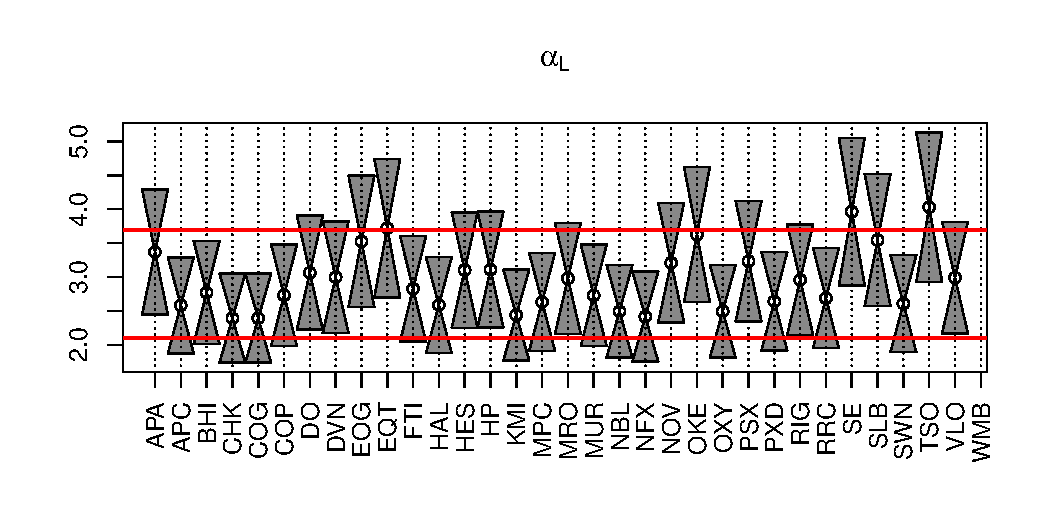
\includegraphics[width=\textwidth, trim={0, 0.8cm, 0, 2cm}, clip]
    {Energy_lower.pdf}
  \end{minipage}
  \begin{minipage}{1.0\linewidth}
    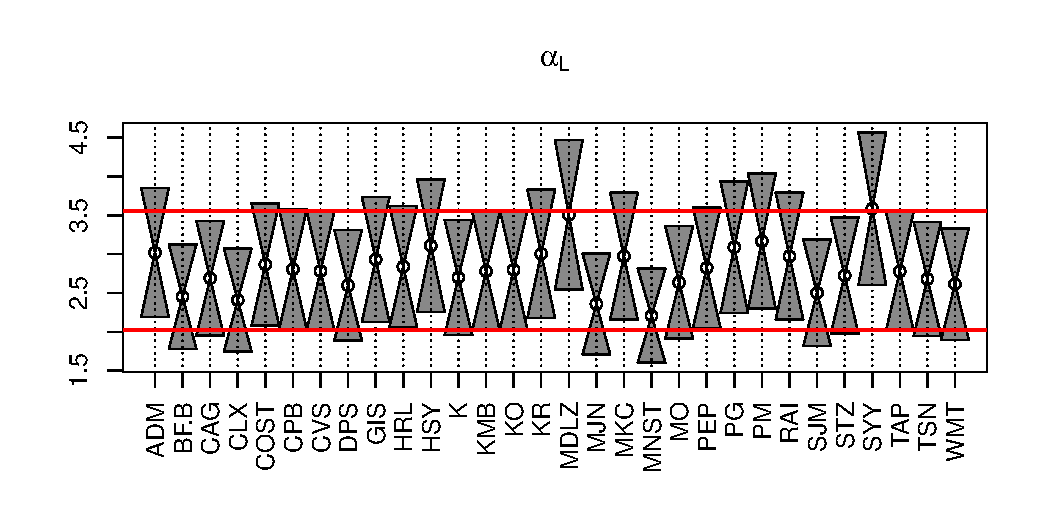
\includegraphics[width=\textwidth, trim={0, 0.8cm, 0, 2cm}, clip]
    {Consumer_Staples_lower.pdf}
  \end{minipage}
  \begin{minipage}{1.0\linewidth}
    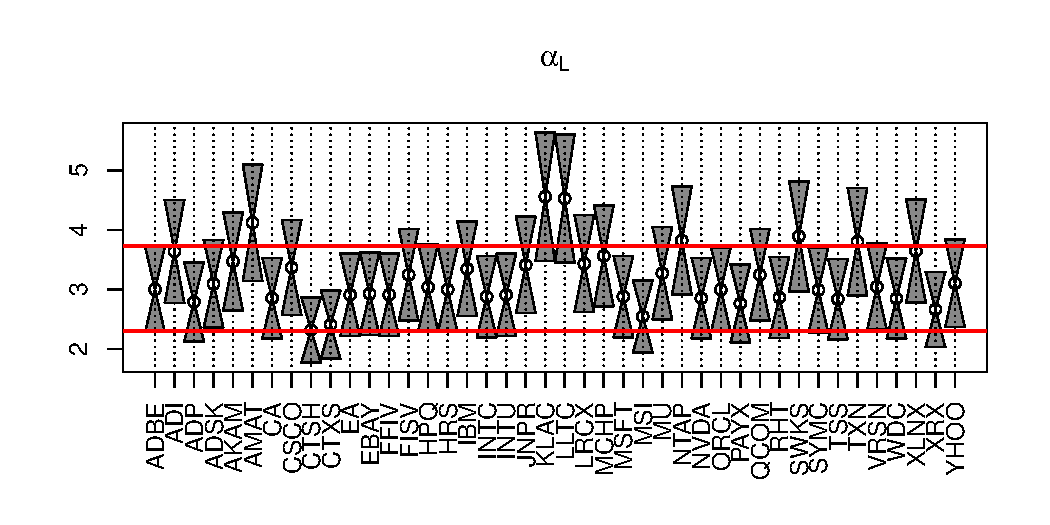
\includegraphics[width=\textwidth, trim={0, 0.8cm, 0, 2cm}, clip]
    {Information_Technology_lower.pdf}
  \end{minipage}
  \caption{\small Hill estimates of lower tail indices of
    daily return series in sectors of Standard \& Poor
    500 index. The figures from top to bottom are ``Energy'',
    ``Consumer Staples'' and ``Information Technology'' sectors.
    Each circle coresponds to a Hill estimate; the grey
    triangles above and below it mark the 97.5\% and 2.5\% quantiles
    of its approximate normal distribution.
    The low and high red lines mark the median of the 2.5\% quantiles
    and median of the 97.5\% quantiles, respectively.
    The data are from {\it Yahoo Finance} and the labels on
    the horizontal axis are Yahoo symbols of the stocks. The data span
    from 2010-01-01 to 2015-01-01 and comprise $n=1304$
    observations. $k=50$ lower order statistics are used
    for computing $\alpha_n$. 
  }\label{fig:1}
\end{figure}

In Figure~\ref{fig:1} we see that confidence intervals of the Hill
estimates of the losses in the ``Energy'' and ``Consumer Staples''
sectors of the S\& P 500 index, as well as those of a 
large portion of losses in the ``Information Technology'' sector,
overlap. This fact indicates that the returns in each sector may 
have comparable tail indices.

Hoga's test on the change of extreme quantiles
may provide some insight about how similar these tail indices are,
because different tail indices are likely to result in different
extreme quantiles. Nevertheless, changes in the extreme quantiles can
be the result of changed tail indices but can also be the result of
changed scale parameters. Thus we first investigate the scale
parameters of stocks in the same sectors before applying Hoga's test.


\subsection{Hill estimates of lower-tail scale parameters}
\label{sec:HillScaleEstimates}

For convenience, we denote the scale parameter by $A$. It is the
constant $J_*(0)$ in the Taylor expansion \eqref{eq:scale_parameter}.
Hill \cite{hill1975simple} put forward an estimator of $A$ using his
tail index  estimator:
\[
\hat A = {k \over n} X_{(k+1)}^{\hat \alpha}
\]
where $X_{(k+1)}$ is the $(k+1)$-th upper order statistic of the
sequence $X_t$ as defined in section\ref{sec:Hill}. $\hat \alpha$
is the Hill tail index estimator.
Estimates of $A$ of the ``Energy'', ``Consumer Staples'' and
``Information Technology'' sectors of the S\&P 500 index are computed
using this method. The results are shown in figure
\ref{fig:sectors_parameters}, along with estimates obtained
using the hybrid method described in section
\ref{sec:hybrid_estimation}.

%% Hence it is informative to test
%% the hypothesis that the tail indices of these return series are equal.
%% Hoga \cite{Hoga2017} devised tests suitable this purpose. We adopt his
%% approach but use our own implementation. The next section has more
%% details.

%% \subsection{Hill estimates of extreme quantiles}


%% By the design of Hoga's test, the null hypothesis can be
%% rejected due to changed scale parameters instead of changed tail
%% indices. Thus it is useful to apply the Hill scale estimator to the
%% same stock return series.

\subsection{Hoga's Test}
\label{sec:Hoga}

Hoga \cite{Hoga2017} proposed his test for a time series
$\{X_i\}_{i=1}^n$ with tail functions
$\bar F_i(\cdot)$, i.e. $\P(X_i > x) = \bar F_i(x)$. The null
hypothesis is
\begin{hypothesis}
  $\mathcal H_0$: For a given $p$, $\exists t^* \in [t_0, 1 - t_0]$
  such that
  \[
  \bar F_1^{-1}(p) = \bar F_2^{-1}(p) = \cdots =
  \bar F_{\floor{t^* n}}^{-1}(p) \neq
  \bar F_{\ceil{t^* n}}^{-1}(p) = \cdots = F_n^{-1}(p)
  \]
\end{hypothesis}
where $t_0 \in (0, 1/2)$. The alternative hypothesis is that no such
$t^*$ exists. Hoga proposed the following test statistics:
\[
Q_1 = \sup_{t \in [t_0, 1 - t_0]}
\left\{
  {
    \left[
      t (1 - t) \ln\left(
      \hat x_p(0, t)
      \over
      \hat x_p(t, 1)
      \right)
    \right]^2
    \over
    \int_{t_0}^t
    \left[
      s \ln \left(
      \hat x_p(0, s)
      \over
      \hat x_p(0, t)
      \right)
    \right]^2 ds
    +
    \int_{t}^{1 - t_0}
    \left[
      (1 - s) \ln \left(
      \hat x_p(s, 1)
      \over
      \hat x_p(t, 1)
      \right)
    \right]^2 ds
  }
\right\}
\]
Under the null hypothesis, Hoga showed that as $n \to \infty$,
\begin{equation}
  \label{eq:Q1_distr}
  Q_1 \overset{d}{\to}
  \sup_{t \in [t_0, 1 - t_0]} q_t
\end{equation}
where
\[
q_t = 
  {
    [W(t) - t W(1)]^2
    \over
    \int_{t_0}^t [W(s) - {s \over t}W(t)]^2 ds
    +
    \int_{t}^{1 - t_0}
    \left[
      W(1) - W(s) - {1 - s \over 1 - t}
      (W(1) - W(t))
      \right]^2 ds
  }
\]
$W(t)$ with $t \in (0, 1)$ is a standard Brownian motion.

When applied to our problem, We would like to test, first of all,
whether there is a change of tail index in each of two 
series and, if there is no change in either series, whether the two
series have the same tail index. Obviously, for either question, if
the tail index changes, the extreme quantile will change.
For the first question, Hoga's test is directly applicable; for the
second, we concatenate the two series before applying the
test.

Figure \ref{fig:Hoga_Single} shows the test statistics of
stocks in the ``Energy'' and ``Consumer Staples'' sectors of the S\&P
500 index. The null hypothesis here is that the tail index remains the
same througout the selected period of time.
\begin{figure}[htb!]
  \begin{minipage}{0.5\linewidth}
    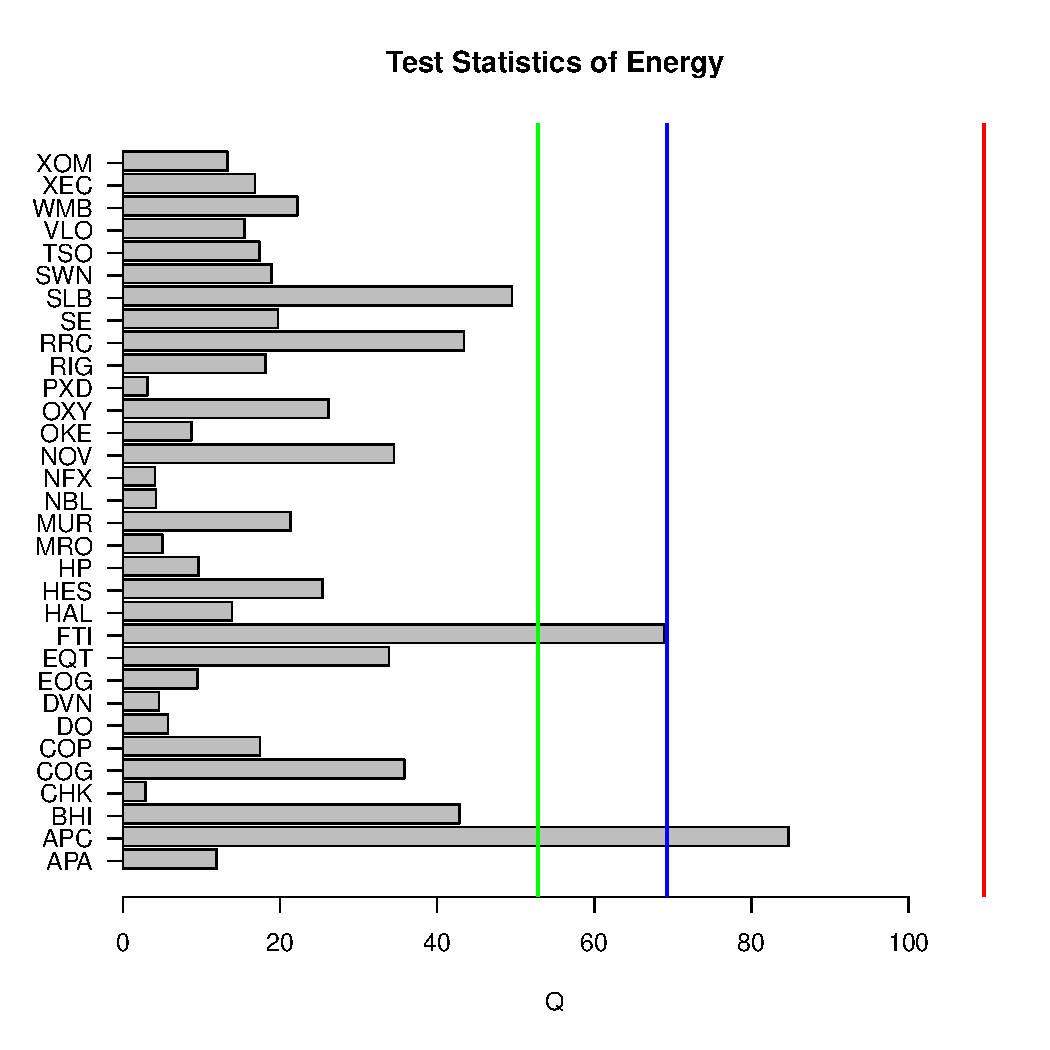
\includegraphics[width=\textwidth]
    {Hoga_Energy_Single.pdf}
  \end{minipage}\hfill
  \begin{minipage}{0.5\linewidth}
    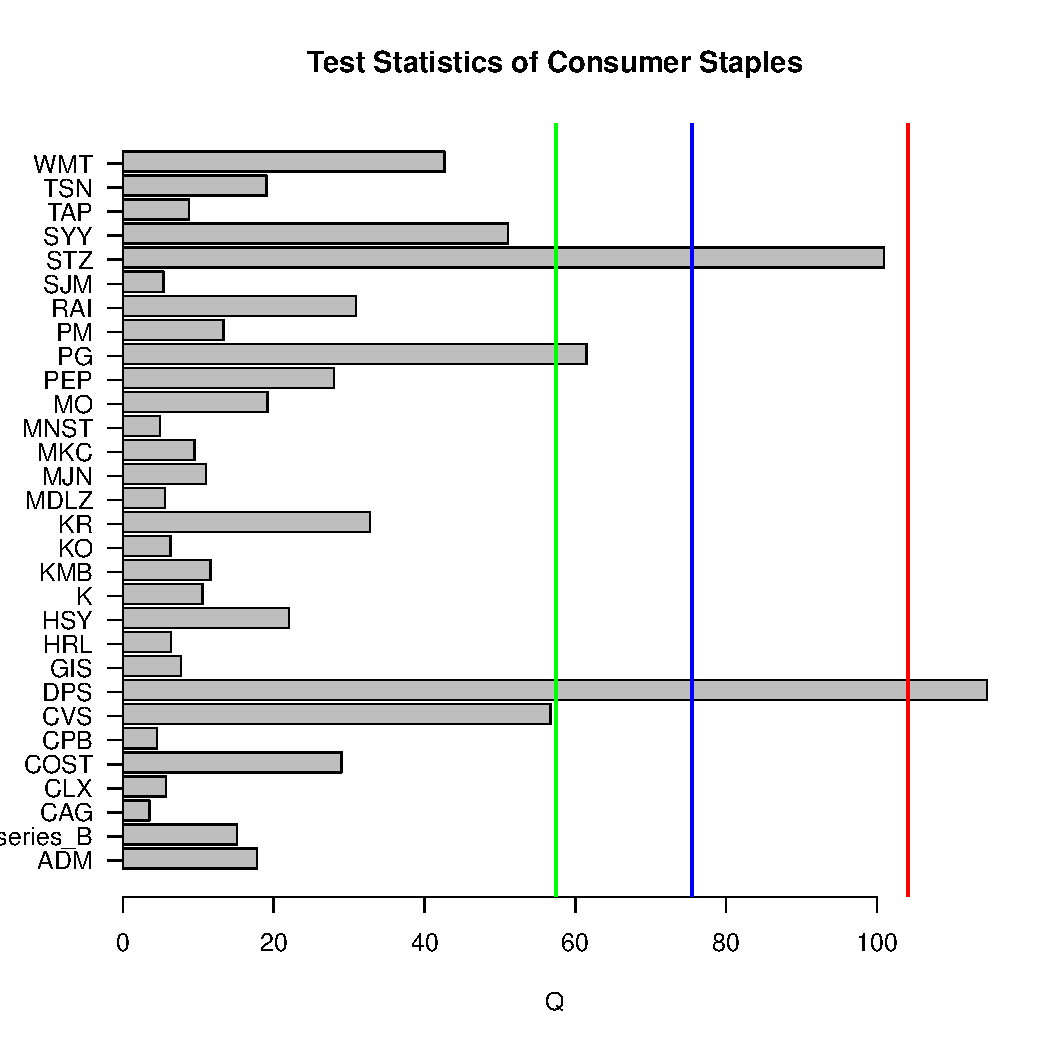
\includegraphics[width=\textwidth]
    {Hoga_Consumer_Staples_Single.pdf}
  \end{minipage}
  \caption{Hoga Test Statistics of stocks in the ``Energy'' and
    ``Consumer Staples'' sectors of S\&P 500. The green, blue and red
    lines are, respectively the 85\%, 90\% and 95\% quantiles of the
    distribution of \eqref{eq:Q1_distr}}.
  \label{fig:Hoga_Single}
\end{figure}

To test whether two series share the same tail index, we concatenate
the two series and apply the Hoga test. For the ``Energy'' and the
``Consumer Staples'' sector, we summarise the results in figure
\ref{fig:Hoga_pair}.
\begin{figure}[htb!]
  \begin{minipage}{0.5\linewidth}
    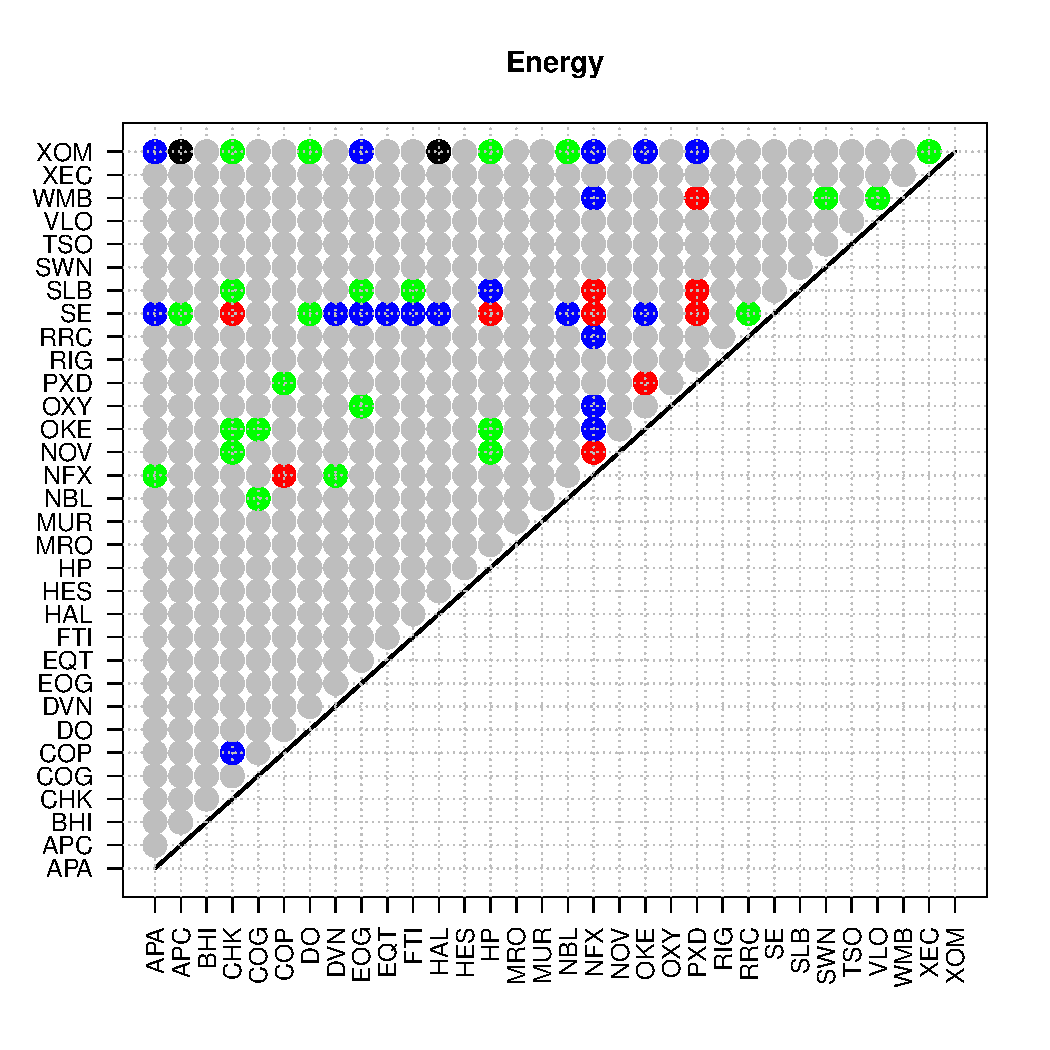
\includegraphics[
      width=\textwidth,
      trim={0.3cm, 1cm, 1cm, 1cm}, clip
    ]{Hoga_Energy_pair.pdf}
  \end{minipage}\hfill
  \begin{minipage}{0.5\linewidth}
    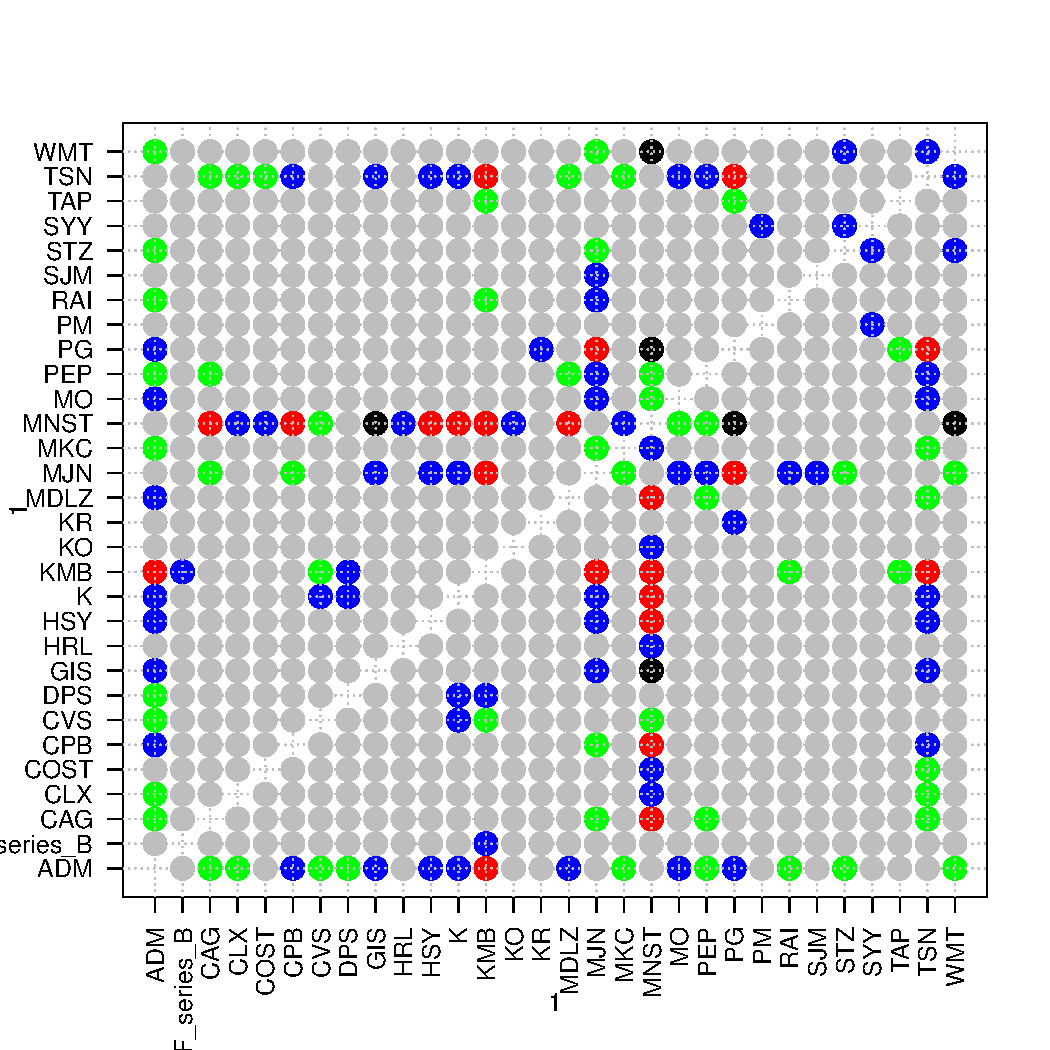
\includegraphics[
      width=\textwidth,
      trim={0.3cm, 1cm, 1cm, 1cm}, clip
    ]{Hoga_Consumer_Staples_pair.pdf}
  \end{minipage}
  \caption{Hoga Test Statistics of stocks in the ``Energy'' and
    ``Consumer Staples'' sectors of
    S\&P 500. The green, blue and red colors represent, respectively,
    exceedances of the 85\%, 90\% and 95\% quantiles of the distribution of
    \eqref{eq:Q1_distr}.
    Grey points stand for pairs for which the test statistic is below
    the 85\% quantile;
    black points represent pairs for which
    computation of the test statistics fails for given precision
    requirements and time limits.}
  \label{fig:Hoga_pair}
\end{figure}
Clearly, these figures show that the null
hypothesis of an equal tail index is rejected for more pairs in the
``Energy'' sector than it is for those in the ``Consumer Staples''
sector. This suggests that lower tail indices of stocks in the
``energy'' sector are more spread out than are those of the ``Consumer
Staples'' sector.

Also observe that while 3 stocks, say A, B and C, test in favor of
relations $\alpha_A = \alpha_B, \alpha_A \neq \alpha_C$, it often
happens that another test on B and C is supportive of $\alpha_B =
\alpha_C$ . This is due to the limited power of the test. Based
on such results, one may guess $\alpha_B$ lies between $\alpha_A$ and
$\alpha_C$. The test is unable to recognize the smaller differences
between $\alpha_A, \alpha_B$ and between $\alpha_B, \alpha_C$.

To have an idea about the power of Hoga's test, we run it on
concatenated samples drawn from t-distributions with different degrees
of freedom. Figure \ref{fig:t_sim_pair} shows the result.
\begin{figure}[htb!]
  \centering
  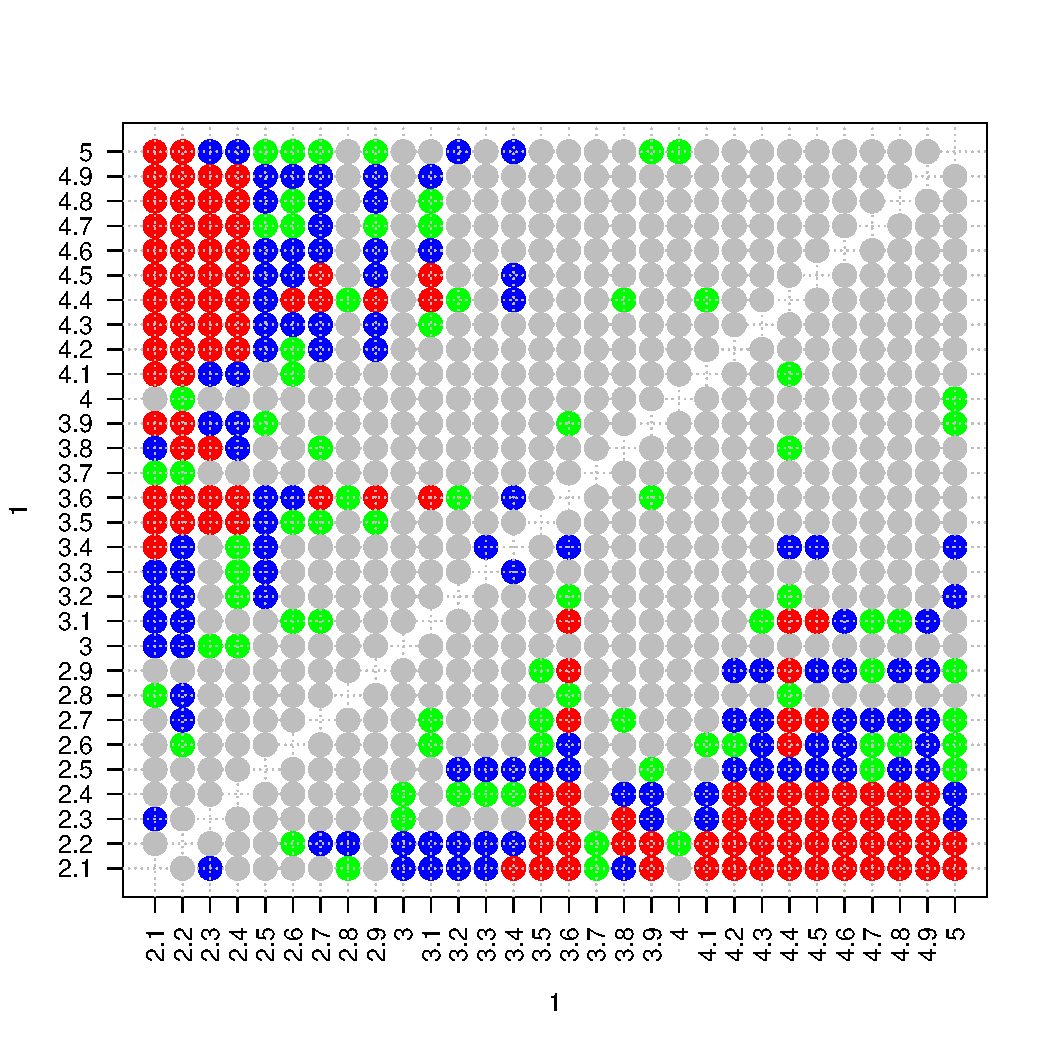
\includegraphics[width=\textwidth, trim={1.0cm 1.5cm 1cm 2cm},
  clip]{t_sim_pair.pdf}
  \caption{Test Statistics of concatenated t-samples with different
    degrees of freedom. Numbers on the axis are the degrees of freedom.}
  \label{fig:t_sim_pair}
\end{figure}
From the figure one can see that the power of the test decreases as
the minimum tail index of a concatenated pair increases.

Also of concern is the distribution of the test statistic under the
null hypothesis. This distribution is only known asymptotically (given
in equation \eqref{eq:Q1_distr}) when the sample size tends to
infinity. The rate at which the finite-sample distribution tends to
\eqref{eq:Q1_distr} is unclear. To find out more about this issue, we
draw samples from the Student's t(3) and t(4) distributions and
compare the empirical distribution of the test statistic $Q_1$ with the
empirical distribution of \eqref{eq:Q1_distr}, which we also obtain by
simulating the Brownian motion $W(t)$. The empirical density functions
are shown in figure \ref{fig:Q1_distr}.
\begin{figure}[htb!]
  \centering
  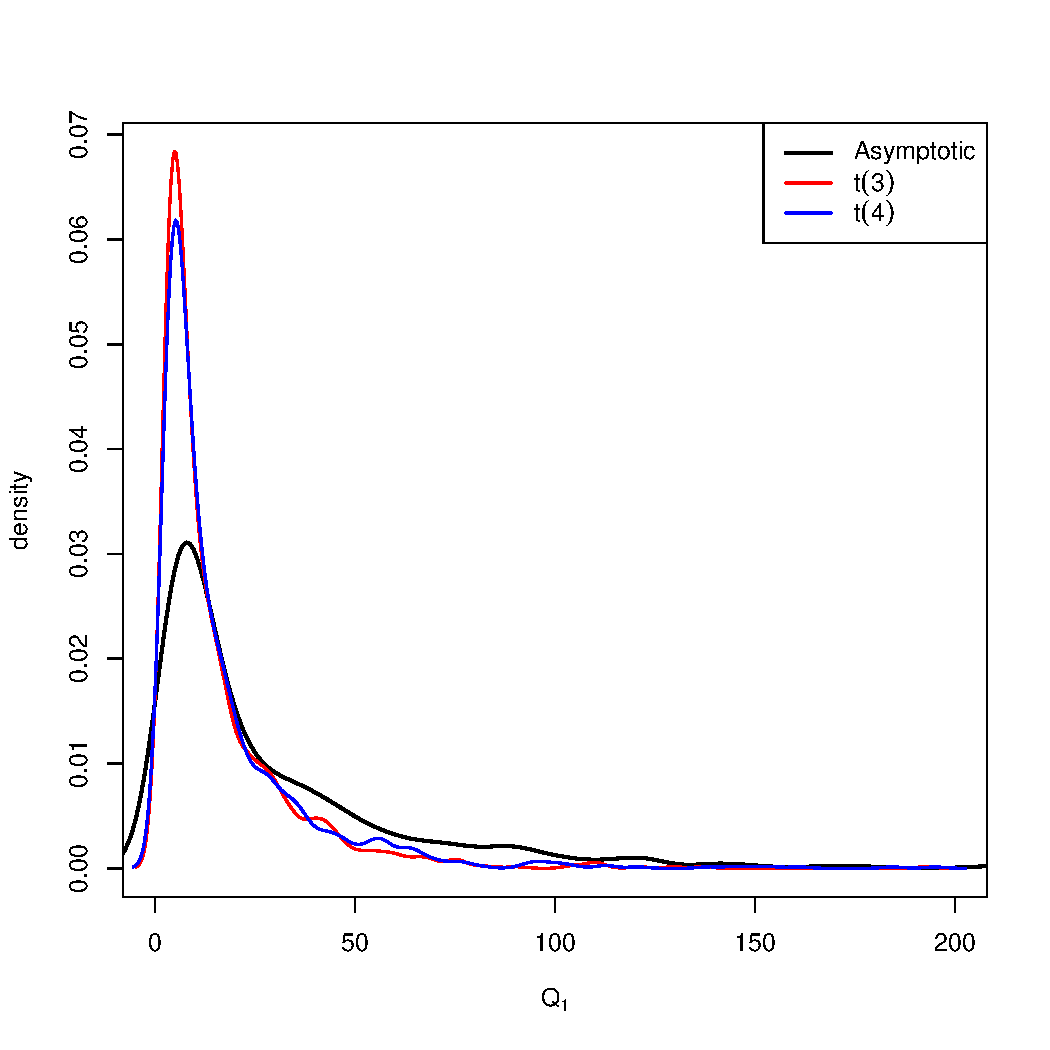
\includegraphics[width=\textwidth]{Hoga_AsymptoticDistribution.pdf}
  \caption{Comparison of the asymptotic distribution with empirical
    distribution of $Q_1$ obtained from Student's t samples. The t
    samples have the same size as the S\&P sectors' data, namely 1304
    observations.}
  \label{fig:Q1_distr}
\end{figure}
As seen in the figure, the asymptotic distribution \eqref{eq:Q1_distr}
assigns significantly more mass to the tail than do the empirical
distributions of size 1304. Table \ref{tab:HogaAsymptotic} lists a few
quantiles of these distributions.
\begin{table}[htb!]
  \centering
  \begin{tabular}{c|c|c|c|c}
    & \multicolumn{4}{c}{Quantiles} \\
    \hline
    Distribution & 80\% & 85\% & 90\% & 95\% \\
    \hline
    Asymptotic & 47.48 & 59.61 & 78.90 & 113.12 \\
    t(3) empirical & 23.30 & 28.27 & 35.04 & 46.75 \\
    t(4) empirical & 25.76 & 31.13 & 38.81 & 56.32
  \end{tabular}
  \caption{Quantiles of the asymptotic and empirical test statistic
    distributions}
  \label{tab:HogaAsymptotic}
\end{table}

\section{Review of multivariate GARCH models:
  same tail index or not}
\label{sec:2}
Many multivariate GARCH models imply a common tail index for all
series under consideration, e.g. the Orthogonal GARCH model of
Alexander and Chibumba (1997) \cite{alexander1997multivariate}, its
generalization GO-GARCH of van der Weide (2002) \cite{van2002go}, as
well as the Full Factor GARCH model of Vrontos et al (2003)
\cite{vrontos2003full} and the Generalized Orthogonal Factor GARCH
model of Lanne and Saikkonen (2007) \cite{lanne2007modeling}. These
models are characterized by their treatment of each series as a linear
combination of factors, and each of the factors is modeled as a GARCH
process. As a result of this treatment, each and every series under
consideration necessarily has the lowest of the tail indices of its
contributing factors (cf. Mikosch (2013) \cite{Mikosch2013} as well
as Andersen, Davis, Kreiss and Mikosch (2009)
\cite{andersen2009handbook}).

In contrast, several other multivariate volatility models imply, in
general, different tail indices for different series. For example, the
Constant Conditional Correlation (CCC-) GARCH model of Bollerslev
(1990) \cite{bollerslev1990modelling} specifies, for a $d$-dimensional
series $\vec X_t$
\begin{eqnarray}
  \cov(X_{i,t}, X_{j,t}) &=& \sqrt{h_{i,t} h_{j,t}} \rho_{i,j}
  \nonumber \\
  h_{i,t} &=& \omega_i + \sum_{l=1}^q A_{i,l} X_{i, t-l}^2 +
  \sum_{l=1}^p B_{i,l} h_{i, t-l} \label{eq:CCC-GARCH}
\end{eqnarray}
Consider the simple case when $p=q=1$. Assume
$X_{i, t} = \sqrt h_{i,t} Z_{i,t}$, $Z_{i, t}$ are iid for
all $t \in \mathbb Z$, and $\P(|Z_{i,t}| > u)/\P(\sqrt h_{i,t} > u) \to 0$ as
$u \to \infty$. Then the tail index of the stationary distribution of
$X_{i,t}$, call it $\kappa_i$, is given by
\[
\E (A_{i, 1} Z^2 + B_{i, 1})^{\kappa_i / 2} = 1
\]
where $Z \overset{d}{=} Z_{i,t}$.
Provided $(A_{i,1}, B_{i,1}) \neq (A_{j,1}, B_{j,1})$, it is clear
$\kappa_i \neq \kappa_j$.

As an extension to the CCC-GARCH model, Jeantheau (1998)
\cite{jeantheau1998strong} proposed his Extended CCC-GARCH by
modifying \eqref{eq:CCC-GARCH} to
\begin{equation}
  \label{eq:ECCC-GARCH}
  \vec h_t =
  \sum_{l=1}^q \mathbf A_{l} (\vec X_{t-l} \odot \vec X_{t-l})
  +
  \sum_{l=1}^p \mathbf B_{l} \vec h_{t-l}
  +
  \vec \omega
\end{equation}
where $\mathbf A_l$ and $\mathbf B_l$ are non-diagonal $d \times d$ matrices
and $\odot$ denotes element-wise multiplication. In the simple case $p=q=1$,
equation \eqref{eq:ECCC-GARCH} reduces to
\begin{eqnarray*}
  h_{i,t} &=&
  \sum_{j=1}^d A_{i,j} X_{j, t-1}^2
  + \sum_{j=1}^d B_{i,j} h_{j, t-1}
  + \omega_i
\end{eqnarray*}
or in vector form
\begin{eqnarray}
  \vec h_t &=& \left[
    \mathbf A \text{diag}(Z_{1, t-1}^2, \dots, Z_{d, t-1}^2) + \mathbf B
    \right] \vec h_{t-1} + \vec \omega
  \label{eq:ECCC-GARCH2}
\end{eqnarray}
On appropriate conditions, \eqref{eq:ECCC-GARCH2} implies the
components of $\vec h_t$ are jointly regularly varying with some index
$\kappa$ as $t \to \infty$. This is a direct result of the Kesten-Goldie
theorem (cf. Kesten (1973)\cite{Kesten1973}). Thus all series under
consideration have the same tail index $\kappa$.

In summary, whether or not a common tail index is shared by all
series is a dividing issue for multivariate GARCH
models. Nevertheless, economic theoretical arguments are supportive of
a common tail index for all series. Therefore, it is important to
gather statistical evidence from financial time series if the issue is
to be settled definitely.

\section{Generalized disappointment aversion}
\label{sec:3}
Routledge and Zin (2010) \cite{routledge2010generalized} define the GDA
preferences over discrete states in their formula (2). A slight extension
is to consider a continuum of possible states. Suppose the state variable
$C$ is continuously supported on $(0, \infty)$ and has distribution
function $G(\cdot)$. The utility function of an agent exhibiting GDA
preferences reads
\begin{equation}
  u(v)= \E u(C) - b \int_{0}^{\delta v}
  \left[ u(\delta v) - u(x) \right] dG(x)\label{11}%
\end{equation}
where $\delta > 0$, and $v>0$. Equivalently
\begin{equation}
  \label{eq:xxie0}
  u(v) = \E u(C) - b \E[u(\delta v) - u(C); C < \delta v]
\end{equation}
Here $v$ can be thought of as the certainty payoff equivalent to the
risky payoff $C$. Note that when $b=0$, 
preferences are expected utility; when $\delta=1$ and $b>0$,
preferences follow Gul's (1991) original disappointment aversion.
An agent guided by this utility function will seek to maximize $u(v)$.

Routledge and Zin \cite{routledge2010generalized} assumed
a power-law utility function of $C$:
\begin{equation}
  \label{eq:power_utility}
  u(C)=\frac{1}{1-\gamma}C^{1-\gamma}%  
\end{equation}
where $\gamma > 0$. For our discussion it suffices that $u(\cdot)$ is
increasing and concave. Before proceeding any further, it is worth
stating the following simple observation:
\begin{lemma} \label{lemma:I}
  Assume distribution function $F(x; \theta)$ parameterized by
  $\theta$ is defined on $x \in (a, b)$, $a, b \in \mathbb R \cup
  \{-\infty, \infty\}$, and in addition $F(x; \theta)$ has density
  function $f(x; \theta)$. Assume function $h(\cdot)$ is defined on
  $(a, b)$, $X \sim F$, $\text{supp}(X) = (a,b)$,
  $\E h(X) < \infty$ and
  \begin{eqnarray*}
    {\partial \over \partial \theta}\left[
      F(b) - F(a)
    \right] = 0 \\
    \left| \frac{\pd f(x, \theta)}{\pd \theta} \right| < \infty
    \quad \forall x \in (a, b)
  \end{eqnarray*}
  \begin{enumerate}
  \item If $h(\cdot)$ is decreasing and $\exists x_0 \in (a, b)$ such that
    $\frac{\pd f}{\pd \theta}(x_0; \theta) > 0$ on $(a, x_0)$ while
    $\frac{\pd f}{\pd \theta}(x_0; \theta) < 0$ on $(x_0, b)$, then
    \[
    \frac{\pd \E h(X)}{\pd \theta} > 0
    \]
  \item If $h(\cdot)$ is increasing and $\exists x_0 \in (a, b)$ such that 
    $\frac{\pd f}{\pd \theta}(x_0; \theta) < 0$ on $(a, x_0)$  while
    $\frac{\pd f}{\pd \theta}(x_0; \theta) > 0$ on $(x_0, b)$, then
    \[
    \frac{\pd \E h(X)}{\pd \theta} > 0
    \]
  \end{enumerate}
\end{lemma}
\begin{remark}
  \label{remark:I}
  Two other cases follow trivially from lemma \ref{lemma:I}:
  \begin{enumerate}
  \item If $h(\cdot)$ is increasing and $\frac{\pd f}{\pd \theta}$
    satisfies the
    same conditions of the 1st case of lemma \ref{lemma:I},
    $\frac{\pd \E h(X)}{\pd \theta} < 0$. This immediately follows
    from applying 1st case of lemma \ref{lemma:I} to $-h(\cdot)$.
  \item By the same argument, if $h(\cdot)$ is decreasing and
    ${\pd f \over \pd \theta}$ satisfies the same conditions of the 2nd case of
    lemma \ref{lemma:I}, ${\pd \E h(X) \over \pd \theta} < 0$.
  \end{enumerate}
\end{remark}
Now for simplicity we assume the investor initially has one unit of
wealth. Let $r > 0$ be the return on the risk free state bond and $X$
be the return on equity. Portfolio weights are $\left(1-\phi\right)$
and $\phi$ respectively. Then
\begin{equation}
  \label{eq:xxie1}
  C(X) = (1 - \phi) e^r + \phi e^X
\end{equation}
Equation \eqref{eq:xxie0} can be re-arranged as
\begin{eqnarray}
u(v) &=& \E u(C) + b \E [u(C); C < \delta v] - b u(\delta v) \P[C < \delta v] \nonumber \\
&=& \E u(C) + b \E [u(C); C < \delta v] - b u(\delta v) F(q) \label{eq:functional}
\end{eqnarray}
where
\begin{eqnarray*}
  q = q(r, \phi) &:=& \ln \left( {
      \delta v - (1 - \phi) e^r
      \over
      \phi
    } \right) = \ln\left(
    e^r + {\delta v - e^r \over \phi}
  \right)
\end{eqnarray*}
Note $C < \delta v$ implies $X < q$. Naturally, if an agent invests in
a risky asset instead of a riskless bond, he expects to obtain a
higher return from the risky asset than he is guarranteed from the
riskless bond. In our notation, this means $\delta v > e^r$, which
implies $q(r, \phi) > r > 0$. The right-hand-side of
\eqref{eq:functional} is a functional of $\phi$ and of the distribution
function of $X$ via \eqref{eq:xxie1}. For convenience we denote it
$\mathcal U(\cdot, \cdot)$, i.e.
\begin{equation}
  \label{eq:U_functional}
  \mathcal U(F, \phi)
  = 
  \E u(C) + b \E [u(C); C < \delta v] - b u(\delta v) F(q(r, \phi))
\end{equation}
In the rest of this section, we use $F(\cdot)$ to denote the
distribution function of $X$ and use $f(\cdot)$ to denote its density
function. Let
\begin{equation}
  \label{eq:G_functional}
  G(F) = \max_{0 < \phi \leq 1} \mathcal U(F, \phi)  
\end{equation}

\subsection{Pareto-distributed equity return}
In this section, we look into the situation when $X$ has a shifted
Pareto distribution. Assume
\begin{equation}
  \label{eq:X_distr}
  F(x) = \left\{
  \begin{array}{ll}
    p \left(
    {K \over K - x}
    \right)^\alpha & x \leq 0 \\
    1 - (1 - p) \left(
    {K' \over K' + x}
    \right)^\beta & x > 0
  \end{array}
  \right.
\end{equation}
Assume $\alpha, \beta > 1$, $0 < p < 1$ and $K > 0$.
We have
\begin{eqnarray}
  && \mathcal U F (\alpha, \beta, K, K', \phi) \nonumber \\
  &=&
  \alpha K^\alpha  p
  \int_{-\infty}^0
  u\left[ (1 - \phi) e^r + \phi e^x \right]
  {1 + b \over (K - x)^{\alpha + 1}} dx
  \nonumber \\
  &&
  \beta K'^\beta (1 - p)
  \int_{0}^\infty
  u\left[ (1 - \phi) e^r + \phi e^x \right]
  {1 + b \1{x < q} \over (K' + x)^{\beta + 1}} dx 
  - b u(\delta v) F(q)
  % &&
  % - b u(\delta v) \left[
  %   1 - (1 - p) {
  %     K'^\beta
  %     \over
  %     (K' + q)^\beta
  %   }
  % \right]
  \label{eq:xxie1.0}
\end{eqnarray}
\begin{theorem}
  \label{thrm:I}
  Suppose functional $G(\cdot)$ is given as \eqref{eq:G_functional},
  function $u(\cdot)$ is increasing and differentiable, then
  \[
  \frac{\pd G(F)}{\pd \alpha} > 0,
  \quad
  \frac{\pd G(F)}{\pd K} < 0
  \]
\end{theorem}
The proof of theorem \ref{thrm:I} is given in secton
\ref{sec:thrmI_proof}.
Since $u(v)$ given in \eqref{eq:xxie1.0} as a
functional of the distribution function of $X$ is increasing with the
lower tail index $\alpha$ and decreasing with $K$, there is a curve of
equal preference on the plane of $(\alpha, K)$. Moving along this
curve in the direction of increasing $\alpha$, one expects the values
of $K$ to increase too, i.e. the estimated values of $\alpha$ and $K$
should appear positively correlated. This is indeed the case in some
real stock return data, e.g. the ``Energy'', ``Consumer Staples'' and
``Information Technology'' sectors of S\&P 500 companies. This is
illustrated in figure \ref{fig:sectors_parameters}.
The confidence bands of the Hill estimates of $\alpha$ of these
sectors are shown in figure~\ref{fig:1}.

By numerically integration and optimization with respect to $\phi$,
the value of $\hat\phi$ can be obtained for given $u(\cdot)$ and given
values of $K, K', \alpha, \beta$. Figures \ref{fig:phi_hat_pareto}
shows the values of $\hat\phi$ for $u(C) = -\frac{C^{-\xi}}{\xi}$ with
$\xi = 1/2, 4$. $\beta=\alpha$ and $K'=K$ in both figures.
\begin{figure}
  \begin{minipage}{0.5\linewidth}
    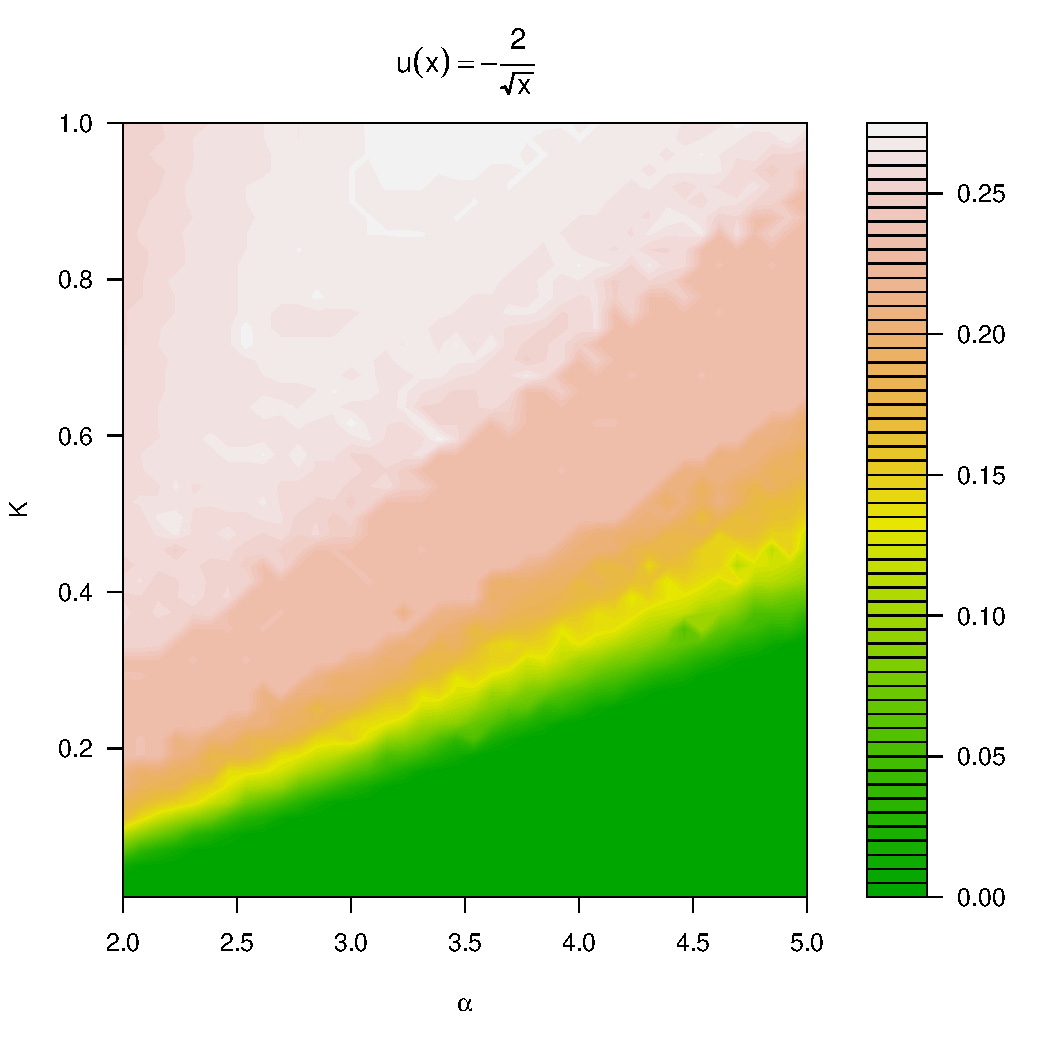
\includegraphics[width=\textwidth]{phi_hat_pareto5e-1.pdf}    
  \end{minipage}\hfill
  \begin{minipage}{0.5\linewidth}
    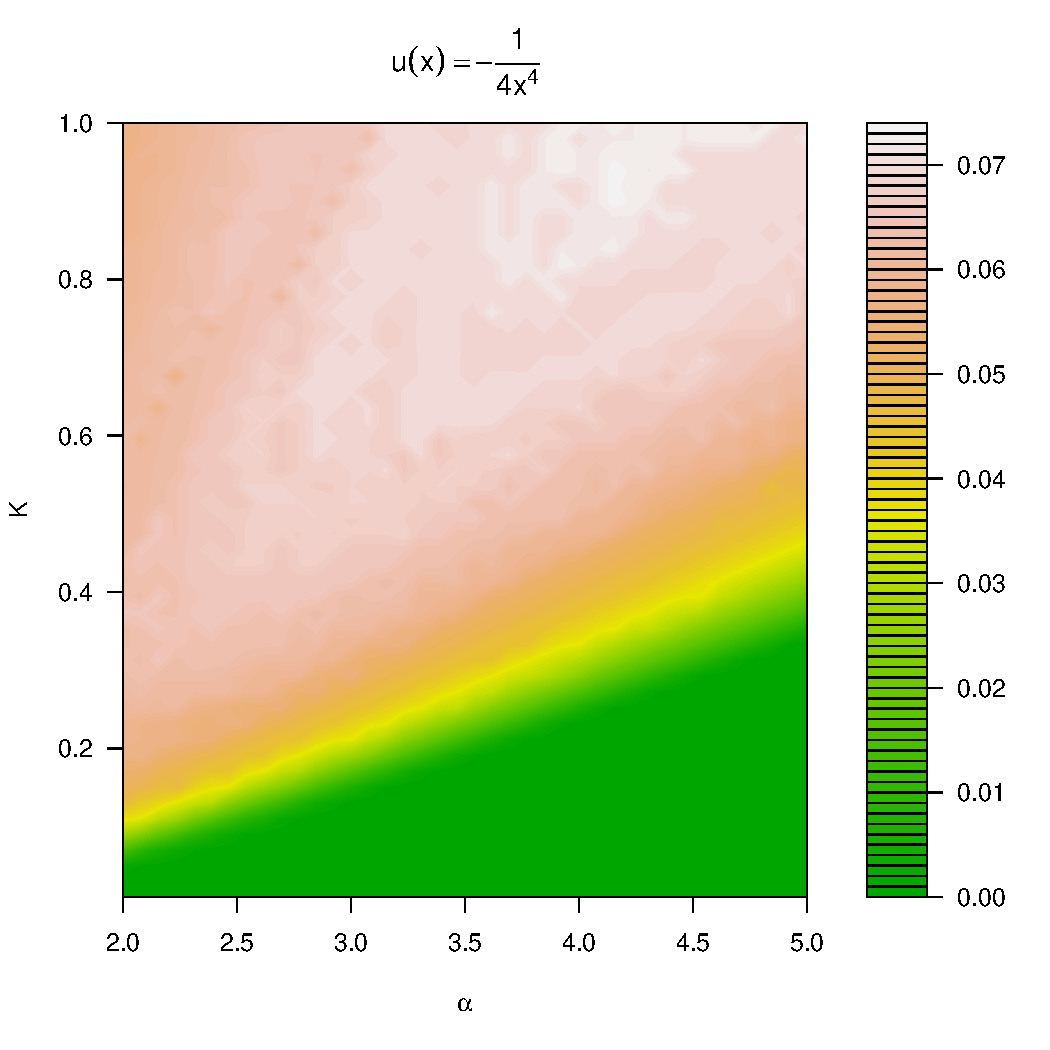
\includegraphics[width=\textwidth]{phi_hat_pareto4.pdf}
  \end{minipage}
  \caption{$\hat\phi$, the optimal equity allocation when the utility
    function is $u(C) = -{C^{-\xi} \over \xi}$ for $\xi = 1/2$
    (left). and $\xi = 1/2$ (right).
  }
  \label{fig:phi_hat_pareto}
\end{figure}

\begin{minipage}{0.5\linewidth}
  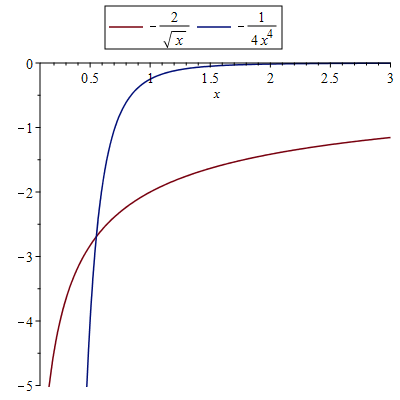
\includegraphics[width=\textwidth]{power_utilities.png}
\end{minipage}\hfill
\begin{minipage}{0.42\textwidth}
  As shown to the left, the power utility function with a small
  $\xi$ grows slower and saturates later than does one with a large
  $\xi$. It represents an agent that is more tolerant of low
  consumption and that seeks wealth more aggressively. In other
  words, he is less risk-averse than is one with a higher $\xi$.
  Such an agent will therefore invest more heavily on the equity as
  is shown in figures \ref{fig:phi_hat_pareto}.
\end{minipage}
Certainly, it rarely happens in practice that the lower- and
upper-tail indices of an equity are equal. Thus, to verify our result
that $G(F)$ is increasing with $\alpha$ and decreasing with $K$, we
need to verify that the 1st integral of \eqref{eq:xxie1.0} with $\phi$
replaced by $\hat\phi$, i.e.
\[
I(\alpha, K) = 
  \alpha K^\alpha  p
  \int_{-\infty}^0
  u\left[ (1 - \hat\phi(\alpha, K)) e^r + \hat\phi(\alpha, K) e^x \right]
  {1 + b \over (K - x)^{\alpha + 1}} dx
\]
is increasing with $\alpha$ and decreasing with
$K$. Figure~\ref{fig:preference_pareto}
shows the values of the above integral when $\alpha$ and $K$ take
a range of values.
\begin{figure}[htb!]
  \begin{minipage}{0.5\linewidth}
    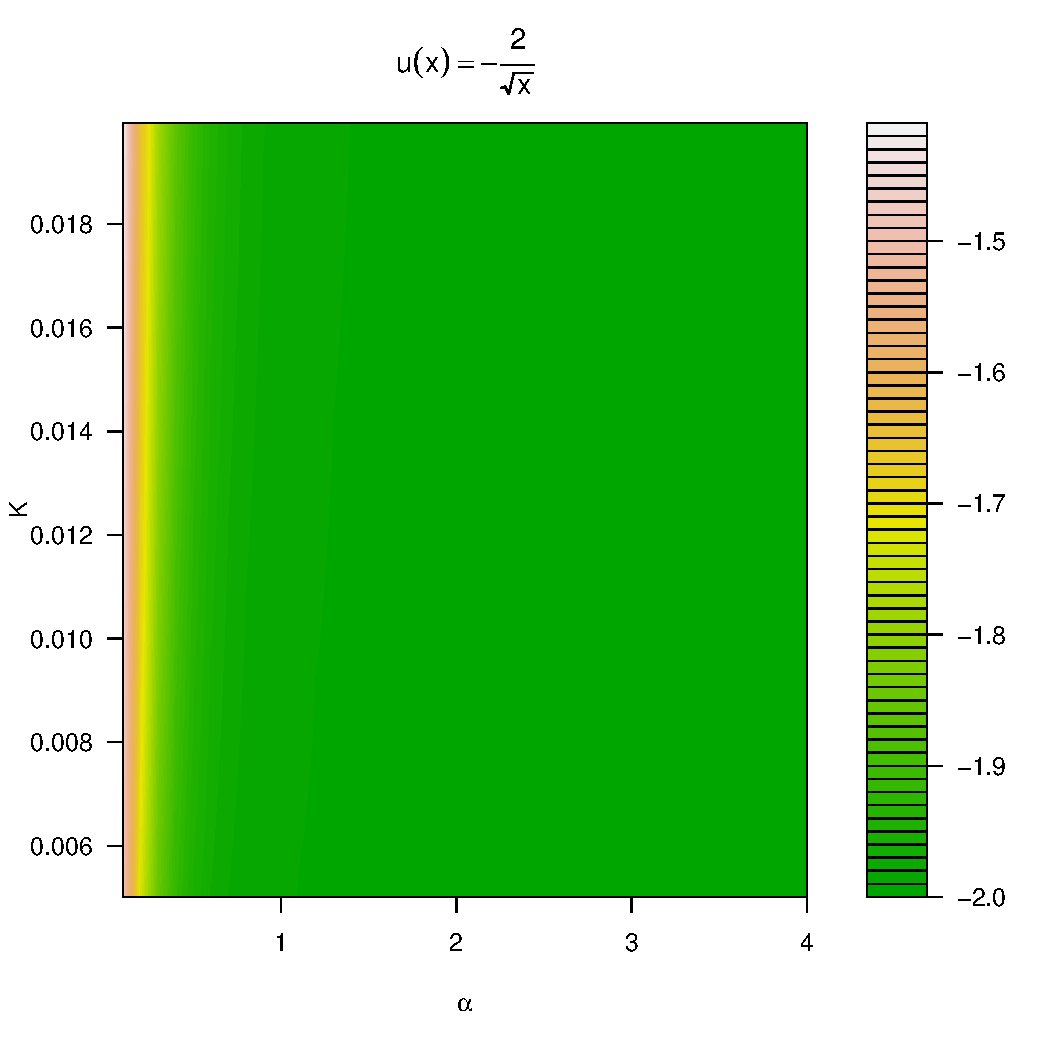
\includegraphics[width=\textwidth]{preference_pareto5e-1.pdf}
  \end{minipage}\hfill
  \begin{minipage}{0.5\linewidth}
    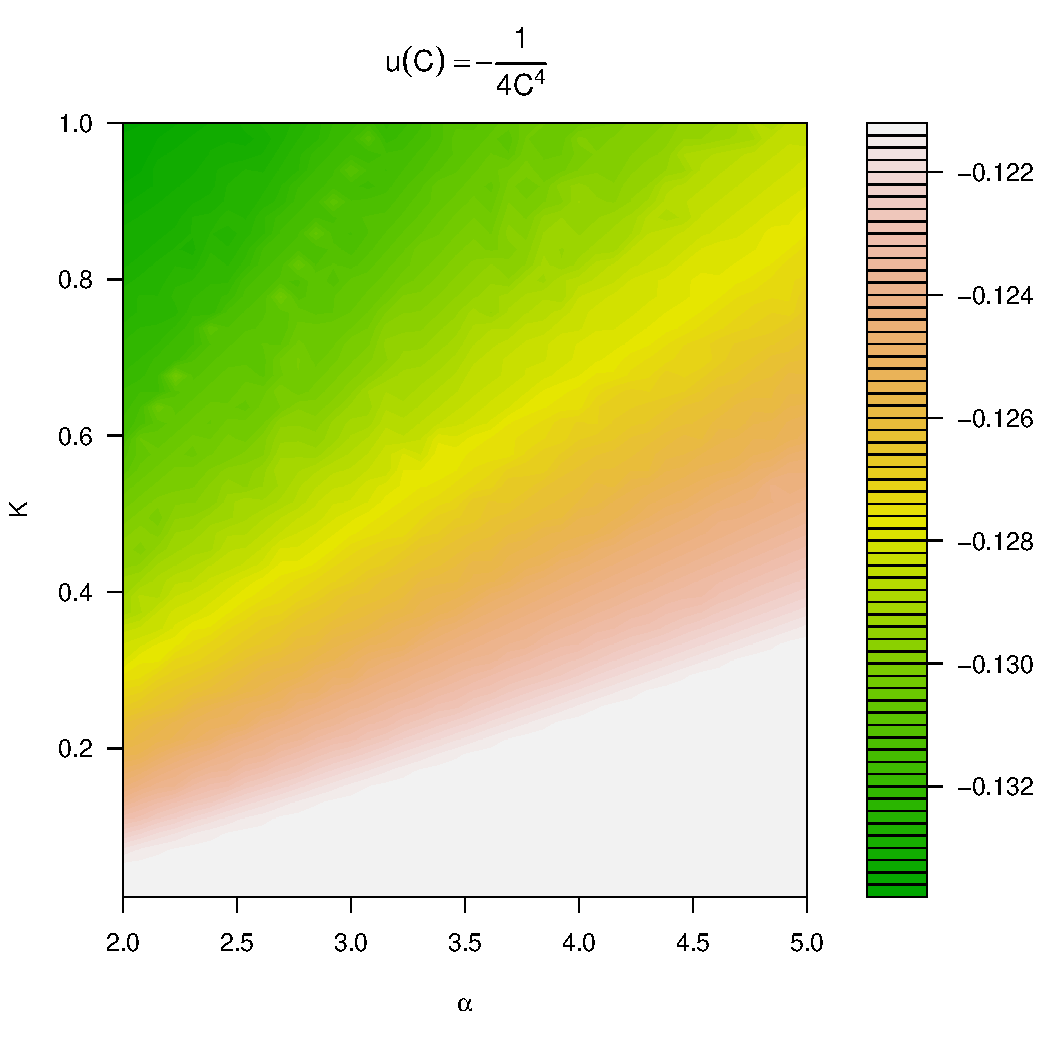
\includegraphics[width=\textwidth]{preference_pareto4.pdf}
  \end{minipage}
  \caption{$I(\alpha, K)$ when the utility function is
    $u(C) = -{C^{-\xi} \over \xi}$ for $\xi = 1/2, 4$.
  }
  \label{fig:preference_pareto}
\end{figure}

\subsection{Hybrid fitting of the shifted Pareto distribution}
\label{sec:hybrid_estimation}
We adopt a hybrid procedure to estimate the parameters of the
distribution function assumed in \eqref{eq:X_distr}: First we
obtain a Hill estimate of the lower-tail indices of an
equity return and fix $\alpha$ in \eqref{eq:X_distr}
to its Hill estimate. Then we estimate $K$ by maximizing
the likelihood function with fixed $\alpha$. Obviously we take only
negative observations and hence condition on $X < 0$. Regularity
conditions on the maximum likelihood estimator are easily checked for
the distribution \eqref{eq:X_distr}.
The density function of $X$ conditional on $X < 0$ is
\[
f_L(x) = {\alpha K^{\alpha} \over (K - x)^{\alpha + 1}}
\]
Clearly, the log-likelihood function of the $K$ parameter is
\[
l(K | X < 0) = \ln(\alpha) + \alpha \ln(K) - (\alpha + 1)\ln(K - X)
\]
where, as is just mentioned, we pre-estimate $\alpha$ with Hill
estimator and regard it as known at this step. With $n$ observations
$X_1, \dots, X_n$, the log-likelihood function of $K$ is
\[
L(K | \forall i=1,2,...,n, X_i < 0) = n \ln(\alpha) + n \alpha \ln(K)
- (\alpha + 1) \sum_{i=1}^n \ln(K - X_i)
\]
To obtain the maximum likelihood estimation, we need to solve the
equation ${\pd L \over \pd K} = 0$, which expands to
\[
{n \alpha \over K} - (\alpha + 1) \sum_{i=1}^n {1 \over K - X_i} = 0
\]
This equation has to be solved numerically.
The Fisher information of $K$ follows as
\begin{eqnarray*}
  I(K) &=& \E\left[ \left( {\partial \over \partial K} l(K | X < 0) \right)^2 \right] \\
  &=& \alpha K^{\alpha - 2}
  \int_{-\infty}^0 {(\alpha x + K)^2 \over (K - x)^{\alpha + 3}} dx \\
  &=& {\alpha \over (2 + \alpha) K^2}
\end{eqnarray*}
So the maximum likelihood estimator, call it $\hat K$, is
asymptotically normal:
\[
\sqrt n (\hat K - K) \to N \left(
  0, \left( 1 + {2 \over \alpha} \right) K^2
\right)
\]

To obtain an estimate of $p$, we use the law of large number:
\begin{eqnarray*}
  p &=& \P(X < 0) = \lim_{n \to \infty}
  {1 \over n} \sum_{t=1}^n \1{X_t < 0}
\end{eqnarray*}
By the central limit theorem,
\begin{eqnarray*}
  \sqrt n \left[
    {1 \over n}\sum_{t=1}^n \1{X_t < 0} - p
  \right] \to N(0, p - p^2))
\end{eqnarray*}


The plots in the 1st column of figure \ref{fig:sectors_parameters}
show the estimates of $K$ alongside the Hill estimates of $\alpha$ of
the ``energy'', ``consumer staples'' and ``information technology''
sectors of the S\&P 500 index;
The plots in the 2nd column show the estimates of $p$ of the same
sectors.

From these figures, one can see that stocks of the ``Energy'' and the
``Information Technology'' sectors generally have larger values of
$p$, meaning their stock prices fall more often than do those in the
``consumer Staples'' sector; Also, the values of $K$ in the ``Energy''
and ``Information Technology'' sectors are larger than those in the
``Consumer Staples'' sector. A larger value of $K$ means, for a given
value of $p$, i.e. a given probability of losses, large losses are
more probable. Thus one can conclude that these two sectors are
considerablly riskier than the ``Consumer Staples'' sector. This is of
course a confirmation of one's economic instinct.

One can also see from figure \ref{fig:sectors_parameters} that, while
the ``Energy'' and the ``Information Technology'' sectors are similar in
riskiness, the correlation between $\alpha$ and $K$ is stronger in
``Energy''. As discussed in the last section, moving along a curve of
equal preference in the direction of increasing $\alpha$, $K$ also
increases. So the strong positive correlation seen in the ``Energy''
sector suggests these stocks might have very similar investor
preferences. This in turn may be attributed to stronger business
relations between the energy enterprises. While two IT companies
may provide a variety of products and services and not depend on each
other, two energy companies are more likely to depend on each other
via relations of supplier and customer or otherwise to compete with each
other if they are on the same link of the chain of energy production
and distribution.

\begin{figure}[htb!]
  \centering
  \begin{minipage}{0.45\linewidth}
    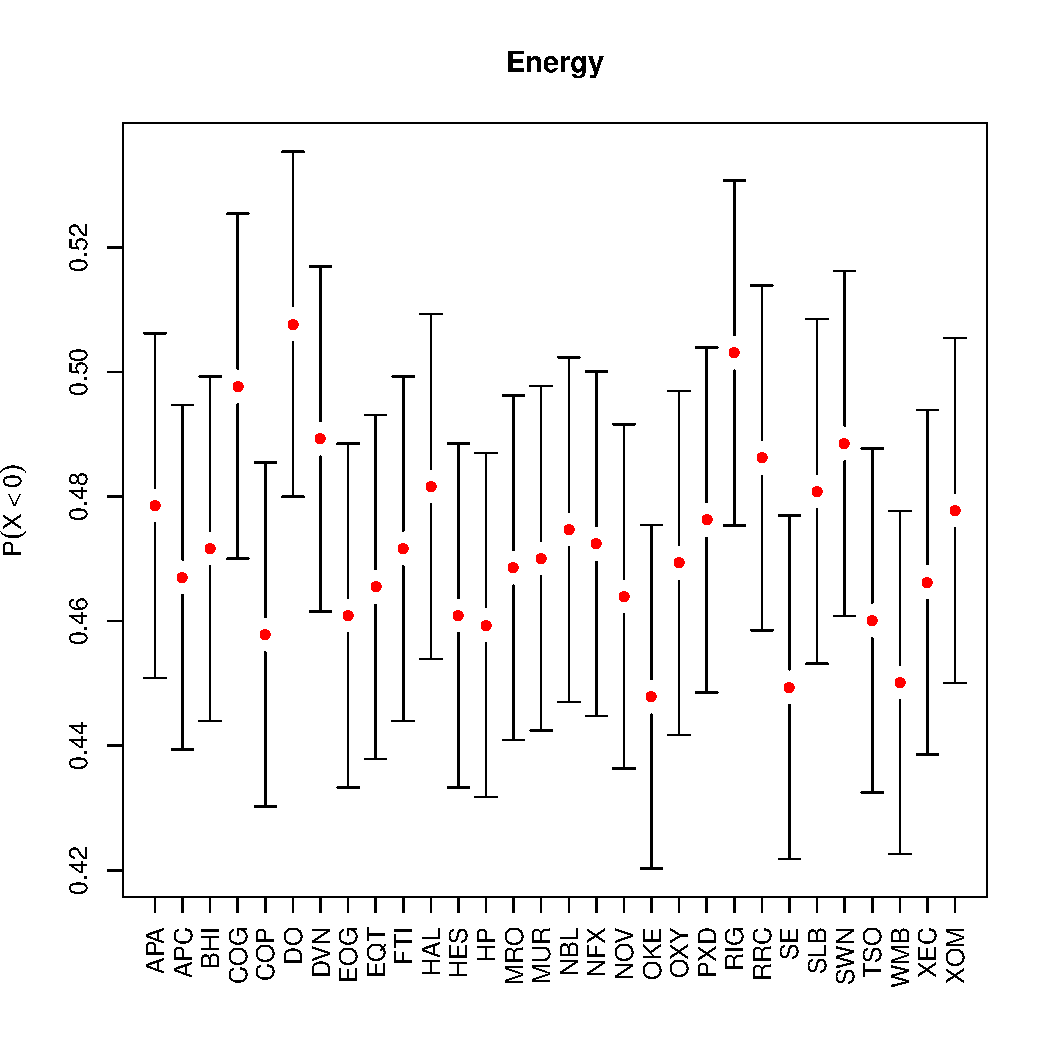
\includegraphics[width=\textwidth]
    {Energy_p.pdf}
  \end{minipage}\hfill
  \begin{minipage}{0.45\linewidth}
    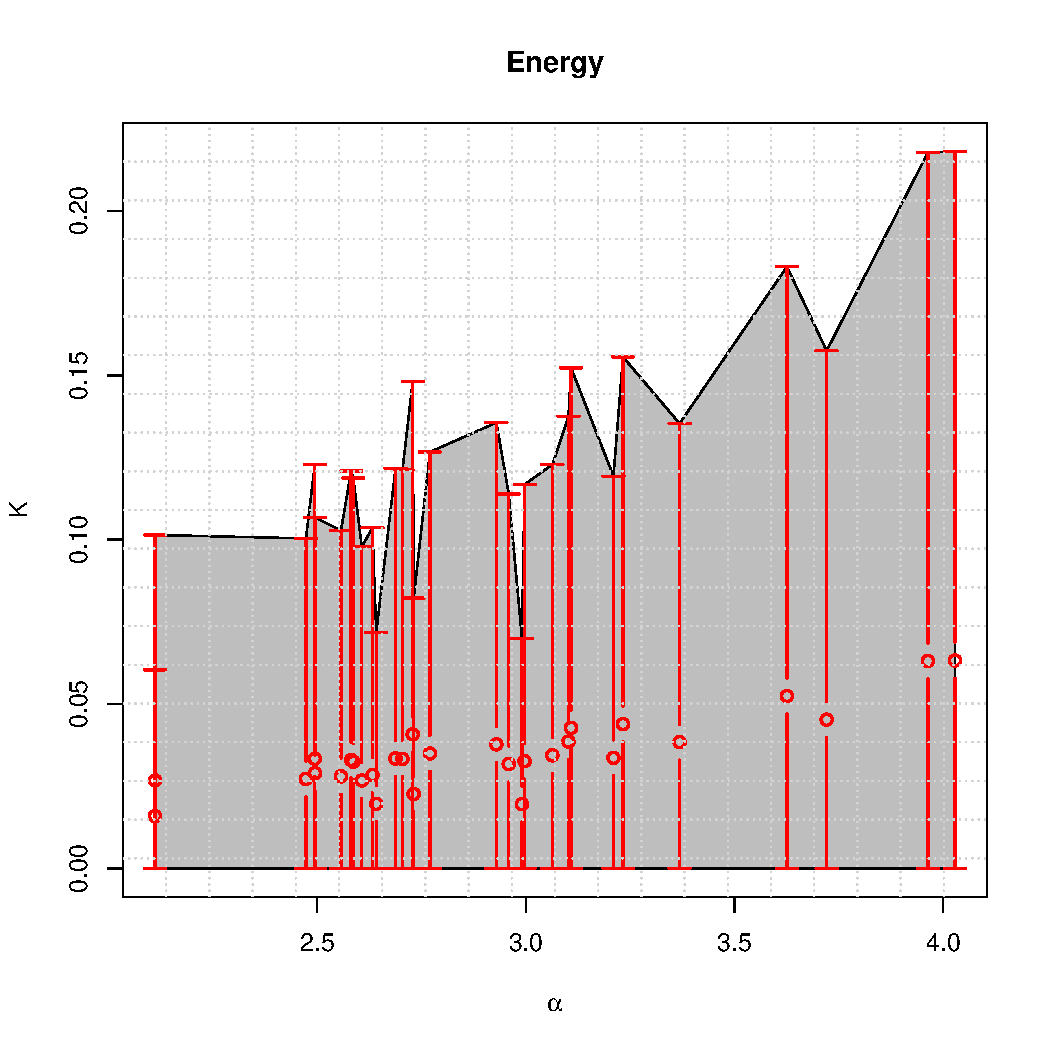
\includegraphics[width=\textwidth]
    {Energy_alpha_K_ci.pdf}
  \end{minipage}
  \begin{minipage}{0.45\linewidth}
    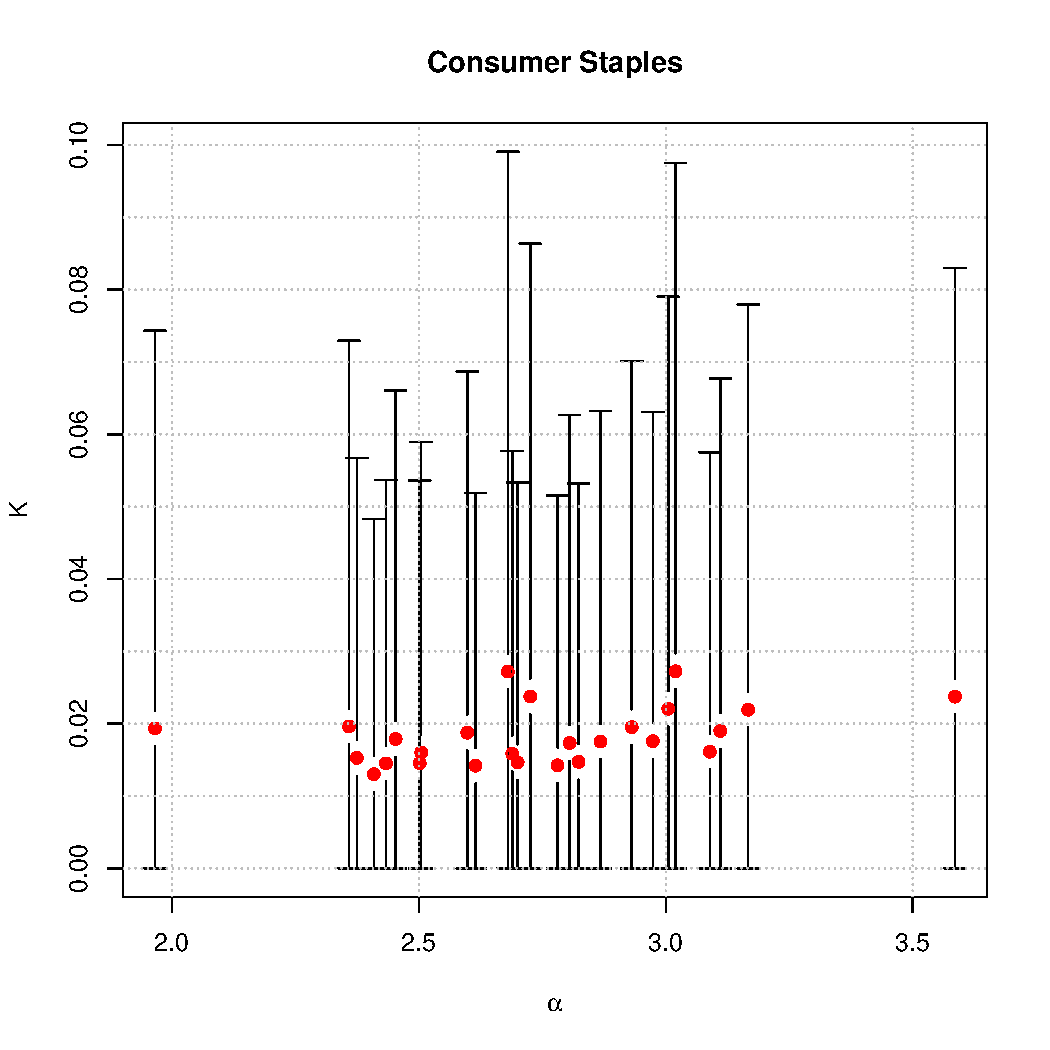
\includegraphics[width=\textwidth]
    {Consumer_Staples_alpha_K_ci.pdf}
  \end{minipage}\hfill
  \begin{minipage}{0.45\linewidth}
    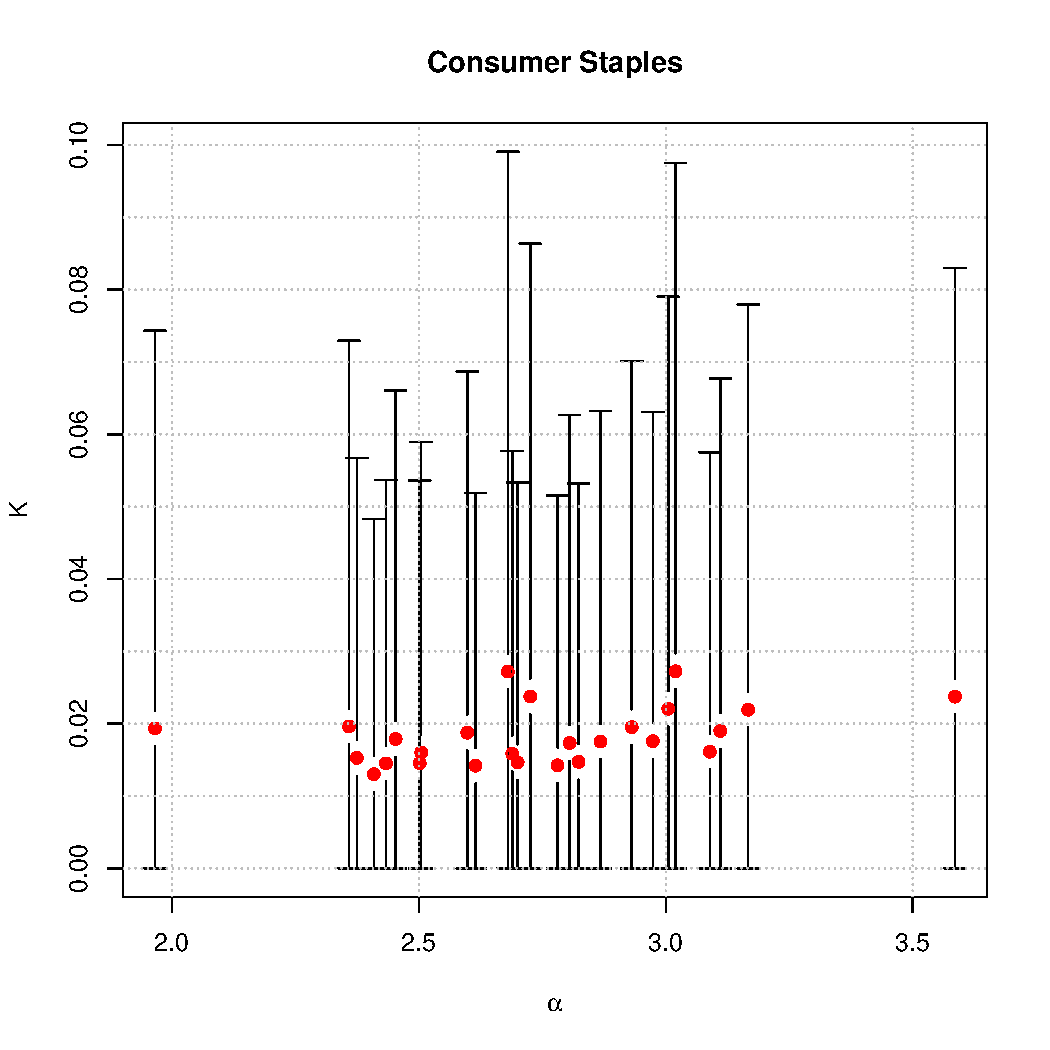
\includegraphics[width=\textwidth]
    {Consumer_Staples_alpha_K_ci.pdf}
  \end{minipage}
  \begin{minipage}{0.45\linewidth}
    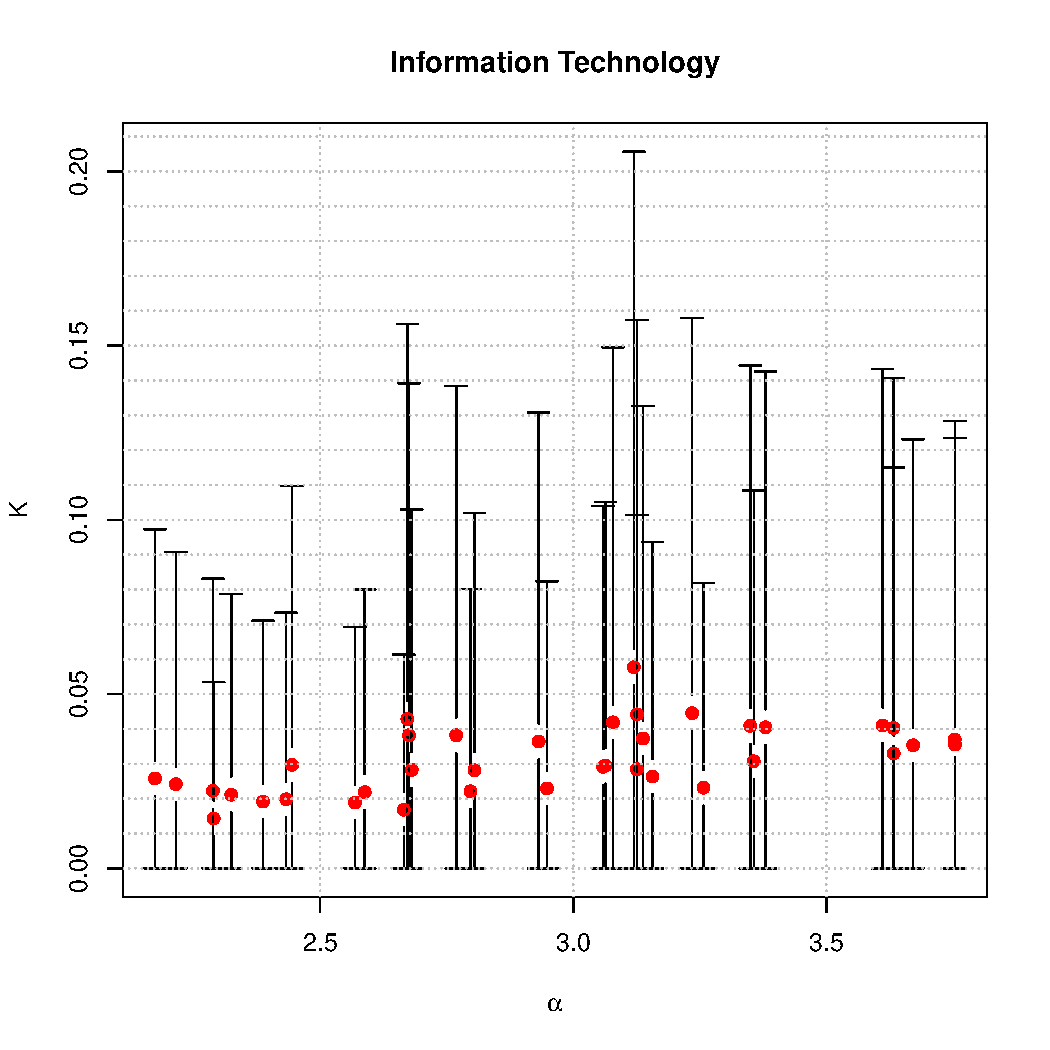
\includegraphics[width=\textwidth]
    {Information_Technology_alpha_K_ci.pdf}
  \end{minipage}\hfill
  \begin{minipage}{0.45\linewidth}
    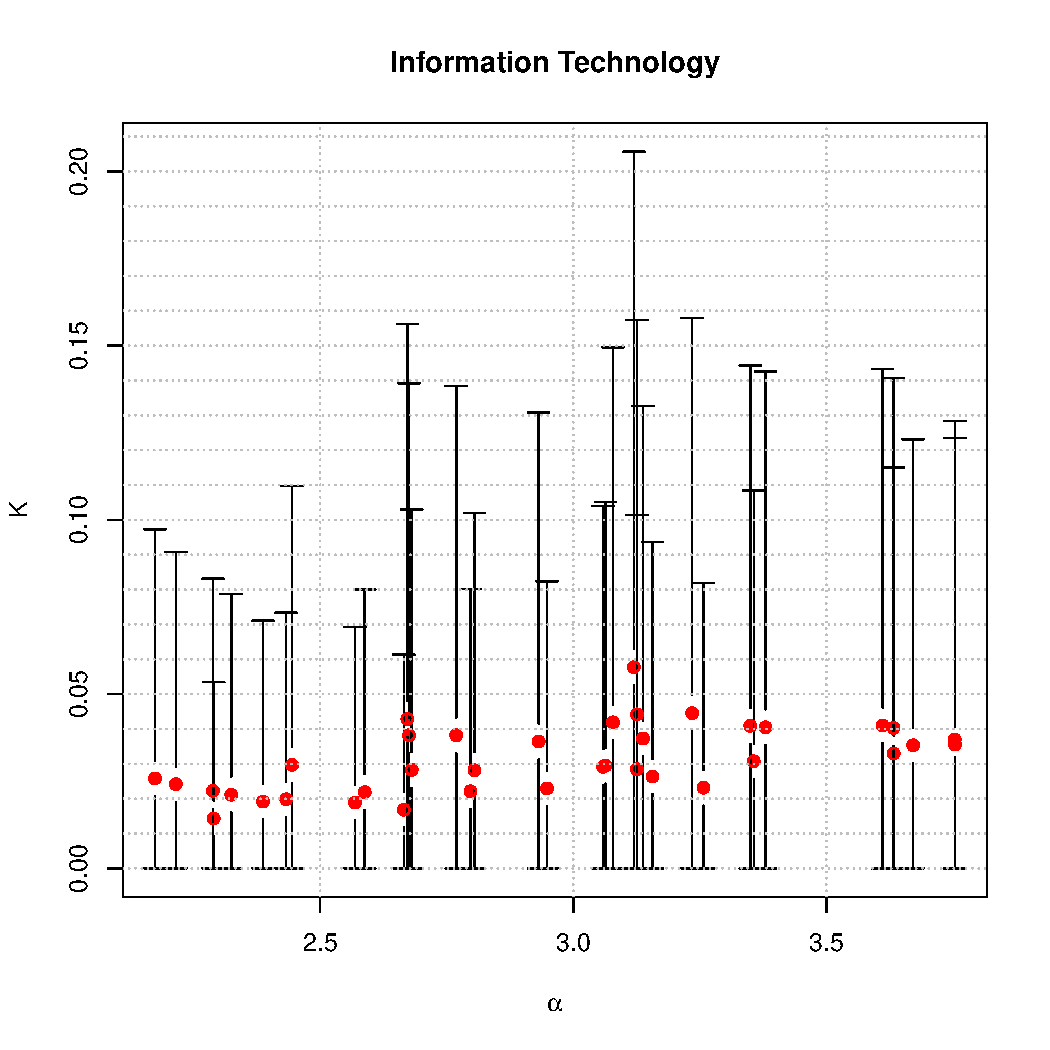
\includegraphics[width=\textwidth]
    {Information_Technology_alpha_K_ci.pdf}
  \end{minipage}
  \caption{\small Estimates of $p$ and $K$ of stocks in sectors of the
    S\&P 500 index. The points are the estimated values; the bars are
    the $2\sigma$ confidence intervals.
  }
  \label{fig:sectors_parameters}
\end{figure}
To compare the maximum likelihood estimates with the results obtained
from Hill's scale estimates, one can re-write the lower-tail
distribution function: For all $x < 0$,
\begin{eqnarray*}
  \P(X < x)
  &=&
  p {K^\alpha \over (K - x)^\alpha} \\
  &=&
  p {K^\alpha |x|^{-\alpha} \over (1 - K/x)^\alpha} \\
  &=&
  p K^\alpha |x|^{-\alpha} \left(
  1 + {\alpha K \over x} + O(|x|^{-2})
  \right)
\end{eqnarray*}
Comparing this expression with \eqref{eq:lower_tail_expansion}, one
can immediately identity $p K^\alpha$ as the scale parameter. Figure
\ref{fig:scale_estimates} compare the estimates obtained
from Hill's scale estimator with those from the $p K^\alpha$ method.

\begin{figure}[htb!]
  \centering
  \begin{minipage}{0.32\linewidth}
    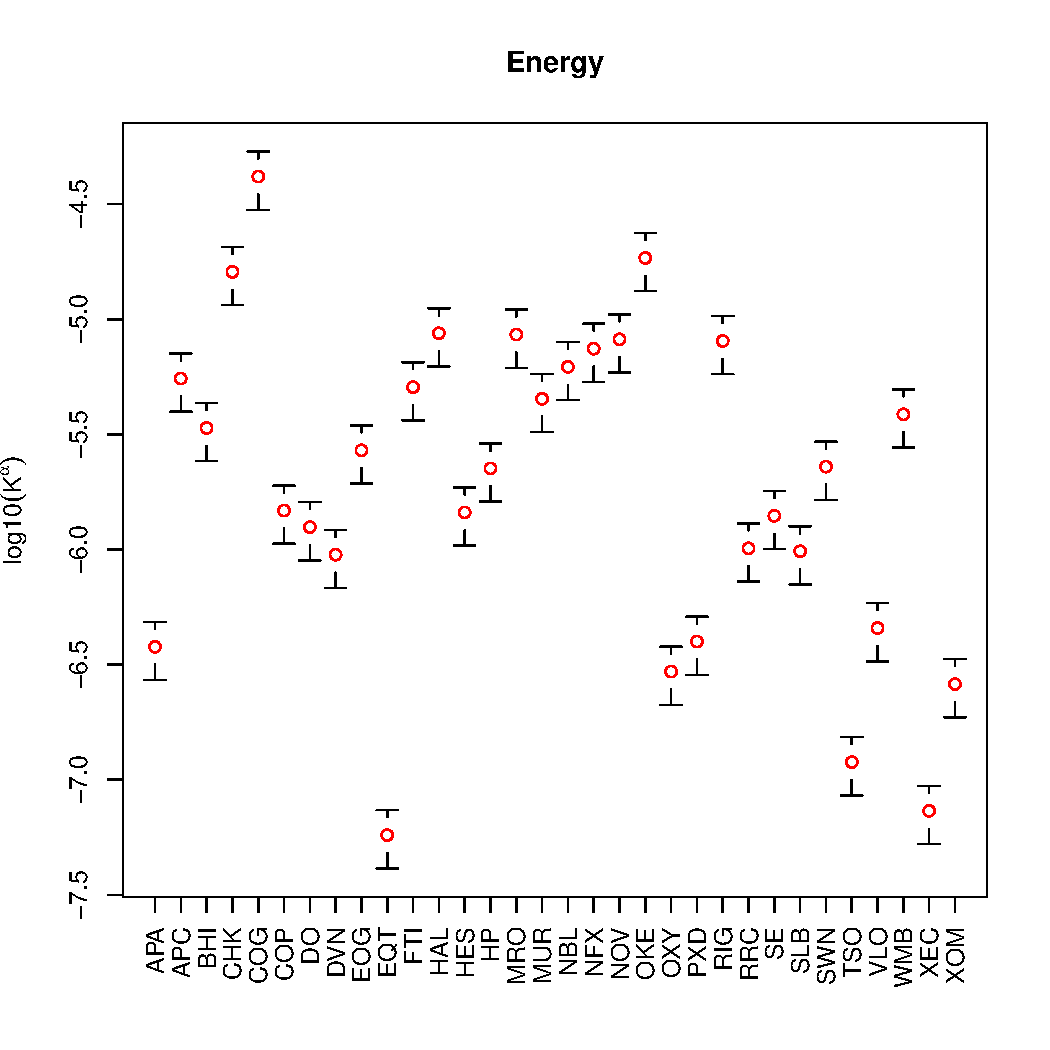
\includegraphics[width=\textwidth]
    {Energy_scale.pdf}
  \end{minipage}
  \begin{minipage}{0.32\linewidth}
    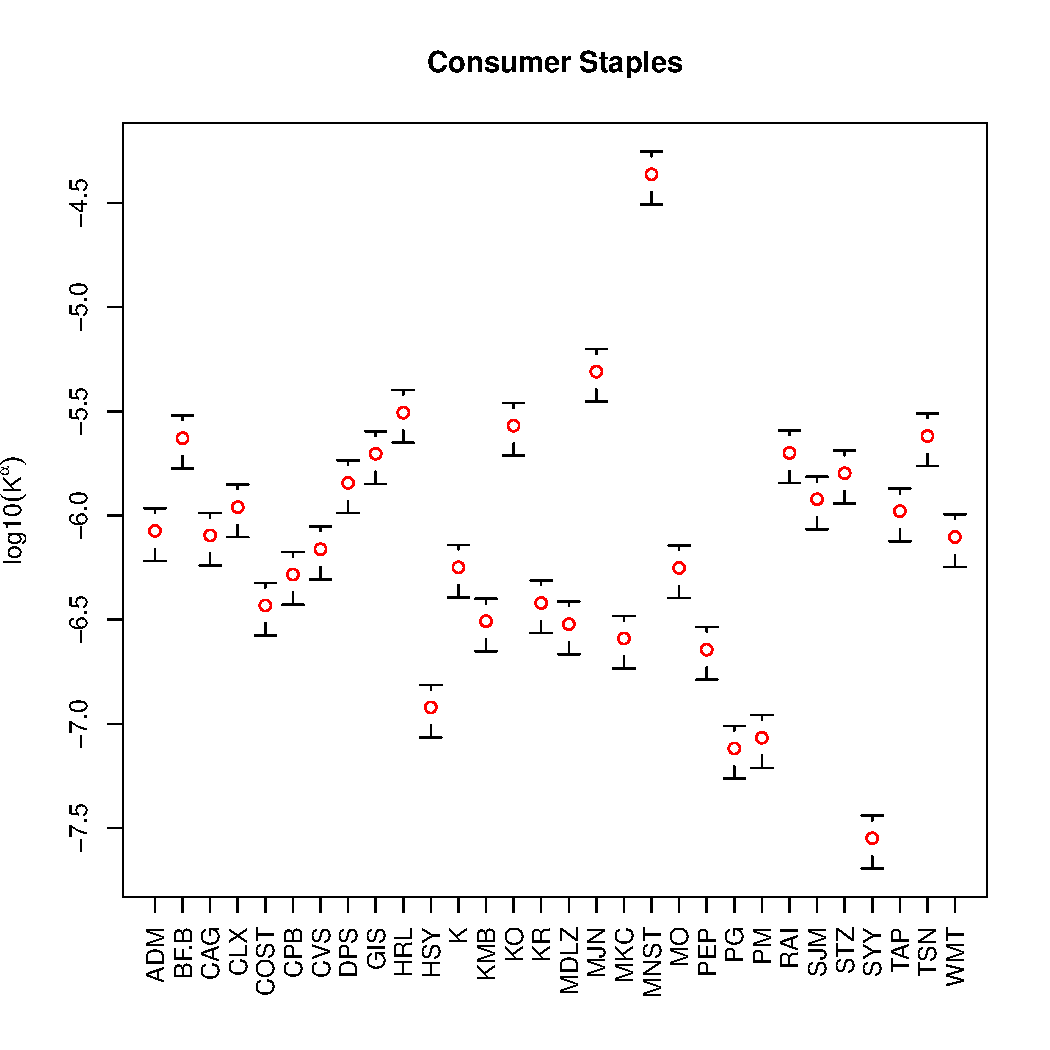
\includegraphics[width=\textwidth]
    {Consumer_Staples_scale.pdf}
  \end{minipage}
  \begin{minipage}{0.32\linewidth}
    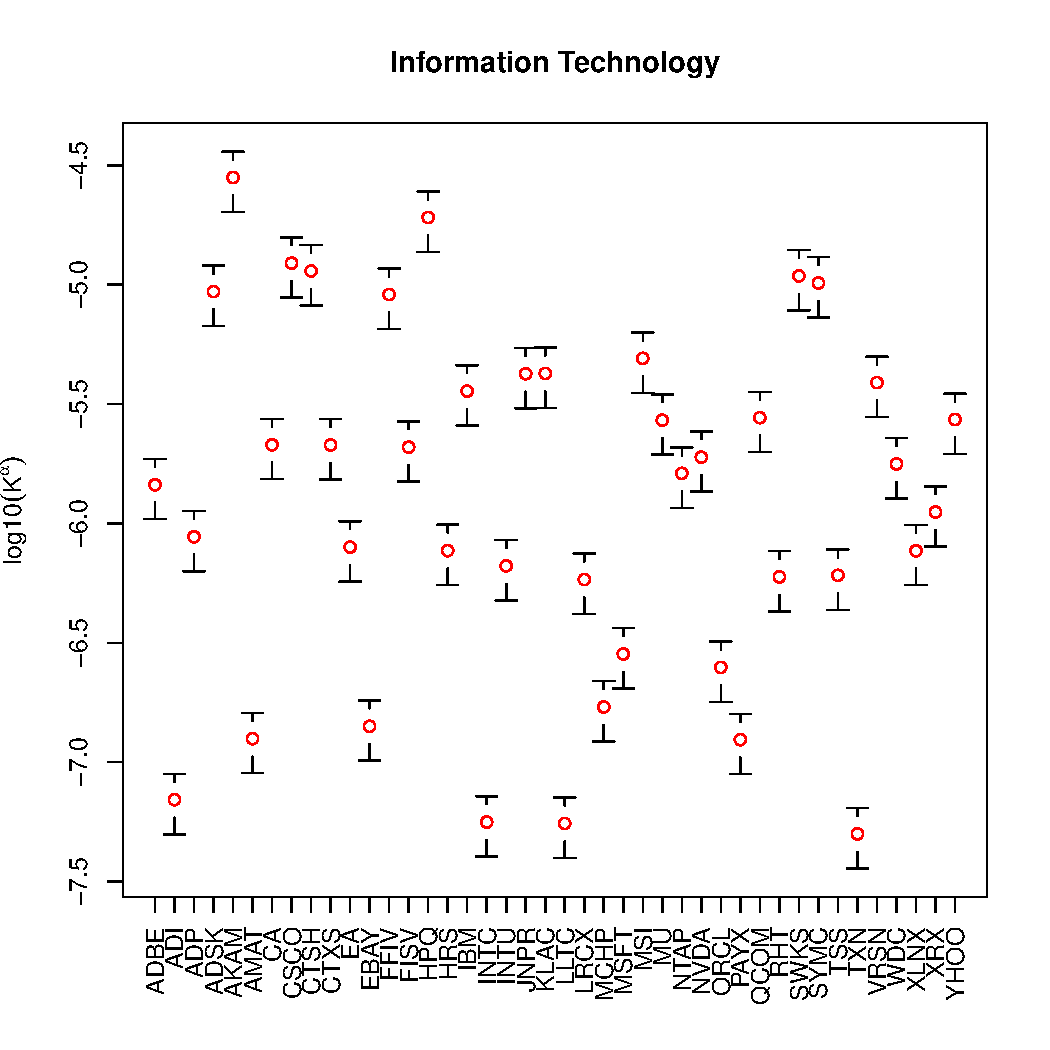
\includegraphics[width=\textwidth]
    {Information_Technology_scale.pdf}
  \end{minipage}
  \caption{\small Scale estimates obtained from Hill's scale estimator
    and from $p K^\alpha$ . Red dots are Hill's scale estimates and
    triangles are $p K^\alpha$ estimates.
  }
  \label{fig:scale_estimates}
\end{figure}

\subsection{Student's t-distributed equity return}
It is a common practice to use Student's t-distribution to model the
stationary distribution of equity returns. So it is of interest to
find out what implications this distribution has when it is combined
with the PDA preference. Formally we assume
\[
f(x; \nu) = c(\nu) \left(
  1 + {x^2 \over \nu}
\right)^{-(\nu + 1)/2}
\]
where $\nu > 1$ and
\[
c(\nu) = {
  \Gamma({\nu + 1 \over 2})
  \over
  \Gamma(\nu/2) \sqrt{\nu \pi}
}
\]
We can write $\mathcal U(F, \phi)$ as
\begin{eqnarray}
  && \mathcal U(F, \phi) \nonumber \\
  &=&
  \int_{0}^{\infty}
  \left[
    u(C(x, \phi)) + (1 + b)u(C(-x, \phi))
  \right]
  f(x, \nu) dx \nonumber \\
  &&
  + b \int_{0}^{q}
  u(C(x, \phi))
  f(x, \nu) dx - b u(C(q, \phi)) F(q, \nu)
  \label{eq:t1}
\end{eqnarray}
where $C(\cdot)$ is defined in \eqref{eq:xxie1}.

\begin{lemma}
  \label{lemma:II}
  There exists $x_0 > 0$ such that ${\pd f \over \pd \nu}(x_0, \nu) = 0$ and
  $\forall x \in (0, x_0), {\pd f \over \pd \nu}(x, \nu) > 0$ and
  $\forall x \in (x_0, \infty), {\pd f \over \pd \nu}(x, \nu) < 0$.
\end{lemma}

\subsubsection{log-utility function}
We first consider the case where the utility function is simply
$u(\cdot) = \ln(\cdot)$. This corresponds to the limiting case of
\eqref{eq:power_utility} as $\gamma \to 0$.

First notice that when $b = 0$, $\mathcal U(F, \phi)$ reduces to
$\E u(C(X, \phi))$. Only the first integral of \eqref{eq:t1} remains.
Its integrand becomes $\ln[C(x, \phi) C(-x, \phi)]$.
Now observe $\ln(C(x, \phi)C(-x, \phi))$ is an increasing function of
$x$:
\begin{eqnarray*}
  {\pd C(x, \phi) C(-x, \phi) \over \pd x}
  &=&
  \phi e^r (1 - \phi) (e^x - e^{-x}) > 0
\end{eqnarray*}
Thus when $b = 0$, by 1st case of remark \ref{remark:I} and lemma
\ref{lemma:II},
${\pd \mathcal U(F, \phi)) \over \pd \nu} < 0$ for all $\phi$. Hence all
investors guided by this utility function would be seeking the
smallest $\nu$, i.e. the heaviest tail in the market. Here note that
Student's t is a symmetric distribution; a heavier tail implies not
only greater down-side risk but also greater up-side potential.

In fact, even when $b > 0$, the same monotonicity property holds. This
is revealed by numerically maximizing $\mathcal U(F, \phi)$ with
respect to $\phi$ for a sequence of selected values of $\nu$. The
results are shown in figure~\ref{fig:phi_hat_U}.
\begin{figure}[htb!]
  % \begin{subfigure}[b]{0.5\linewidth}
  %   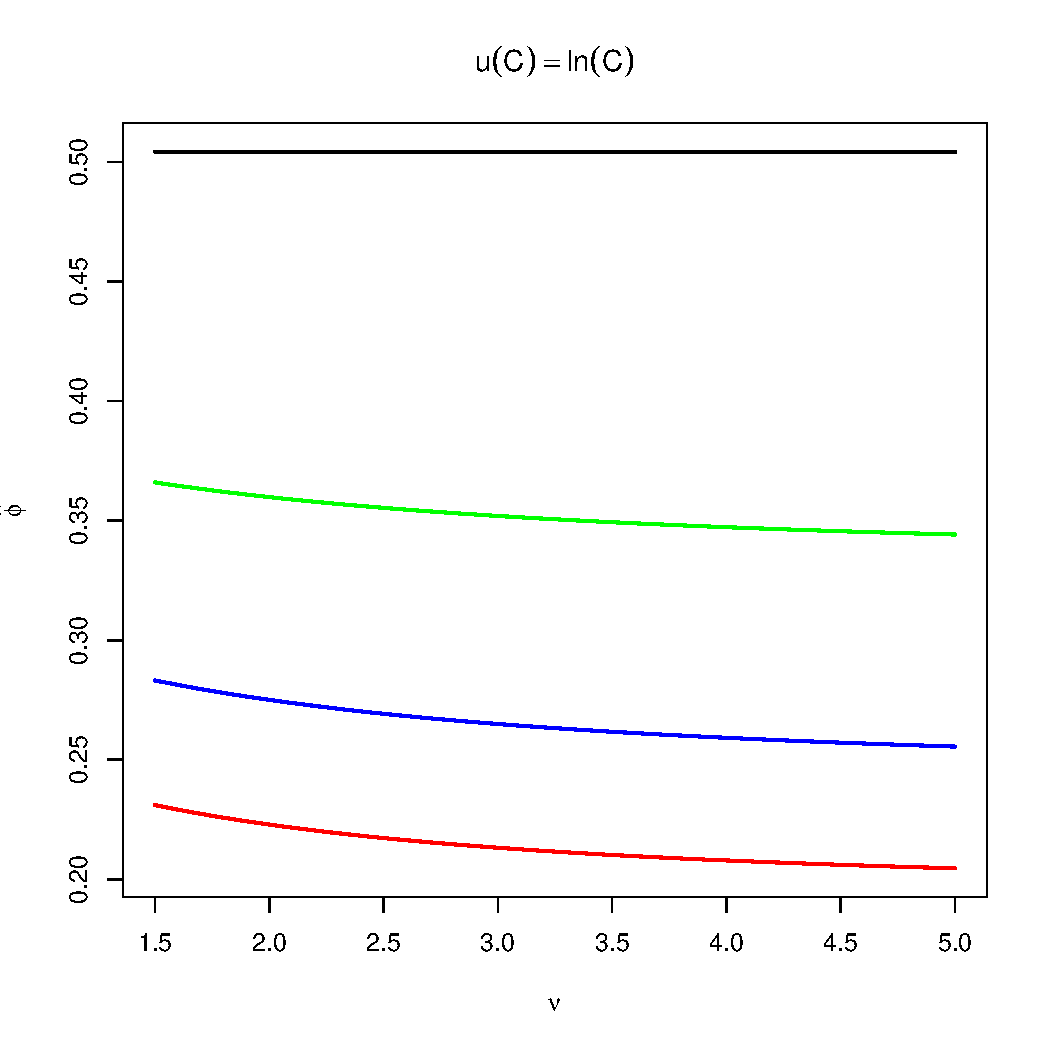
\includegraphics[width=\textwidth]{phi_hat_b_t_log.pdf}
  %   \caption{$\hat\phi(\nu)$ of log-utility function}
  %   \label{fig:phi_hat_t_log}
  % \end{subfigure}
  % \begin{subfigure}[b]{0.5\linewidth}
  %   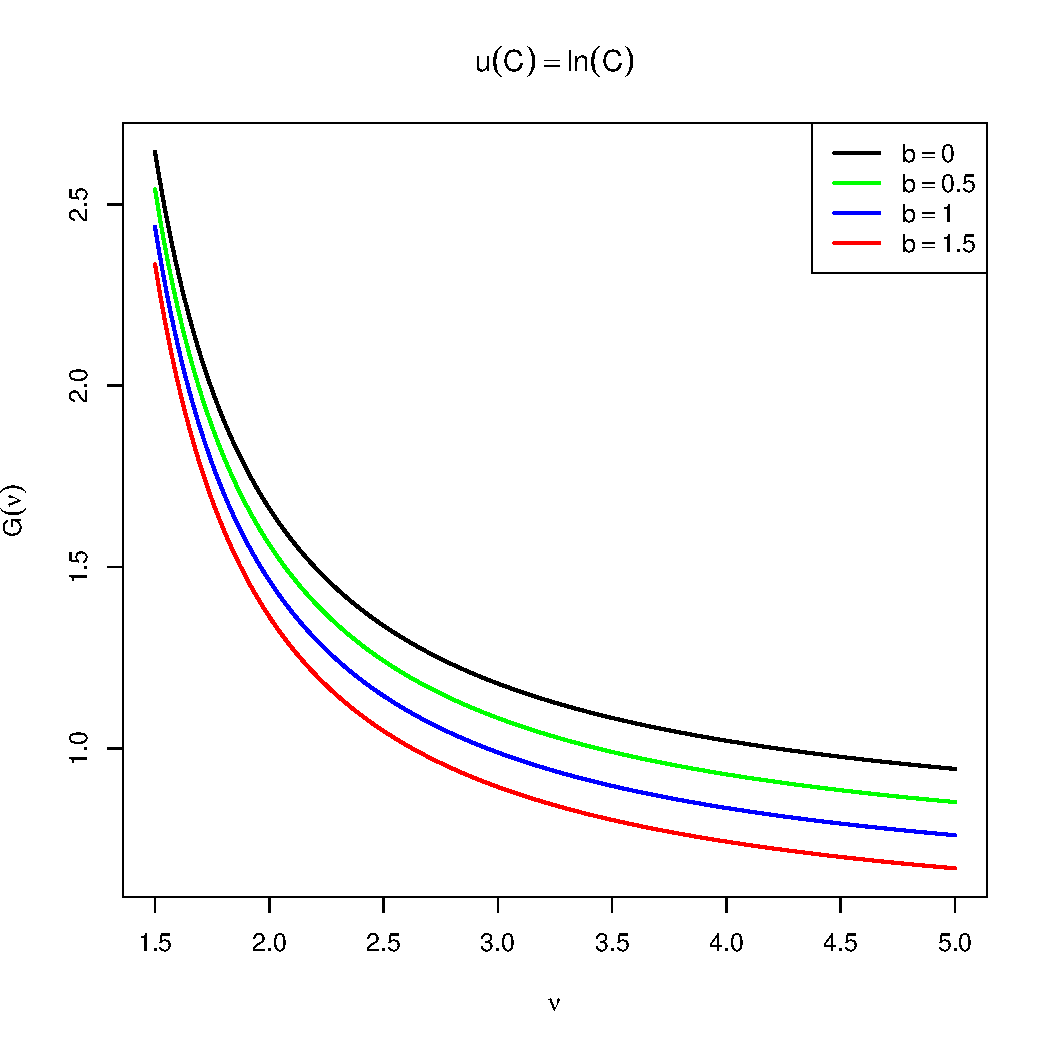
\includegraphics[width=\textwidth]{U_b_t_log.pdf}
  %   \caption{$G(\nu)$ of log-utility function}
  %   \label{fig:U_b_t_log}
  % \end{subfigure}
  % \begin{subfigure}[b]{0.5\linewidth}
  %   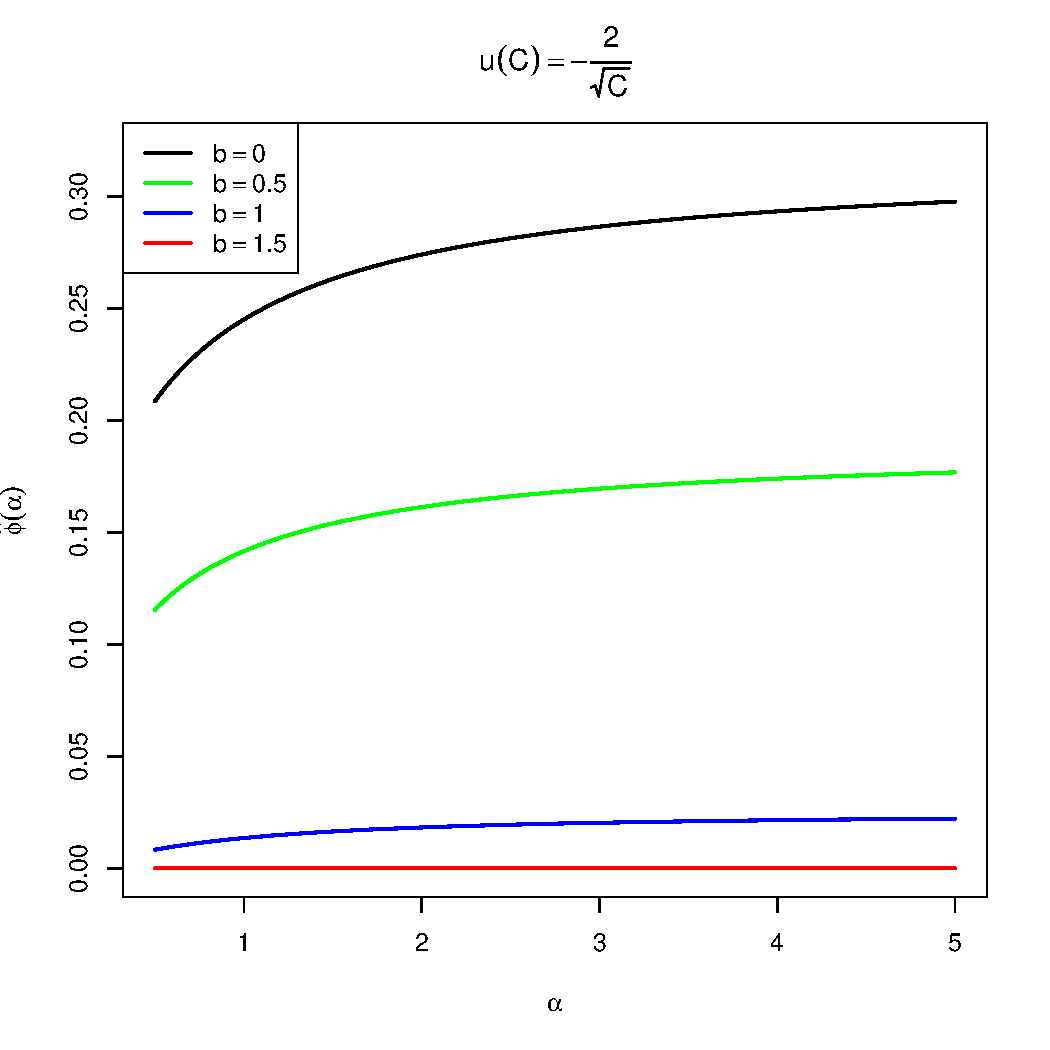
\includegraphics[width=\textwidth]{phi_hat_b_t_power.pdf}
  %   \caption{$\hat\phi(\nu)$ of power-utility function}
  %   \label{fig:phi_hat_t_power}
  % \end{subfigure}
  % \begin{subfigure}[b]{0.5\linewidth}
  %   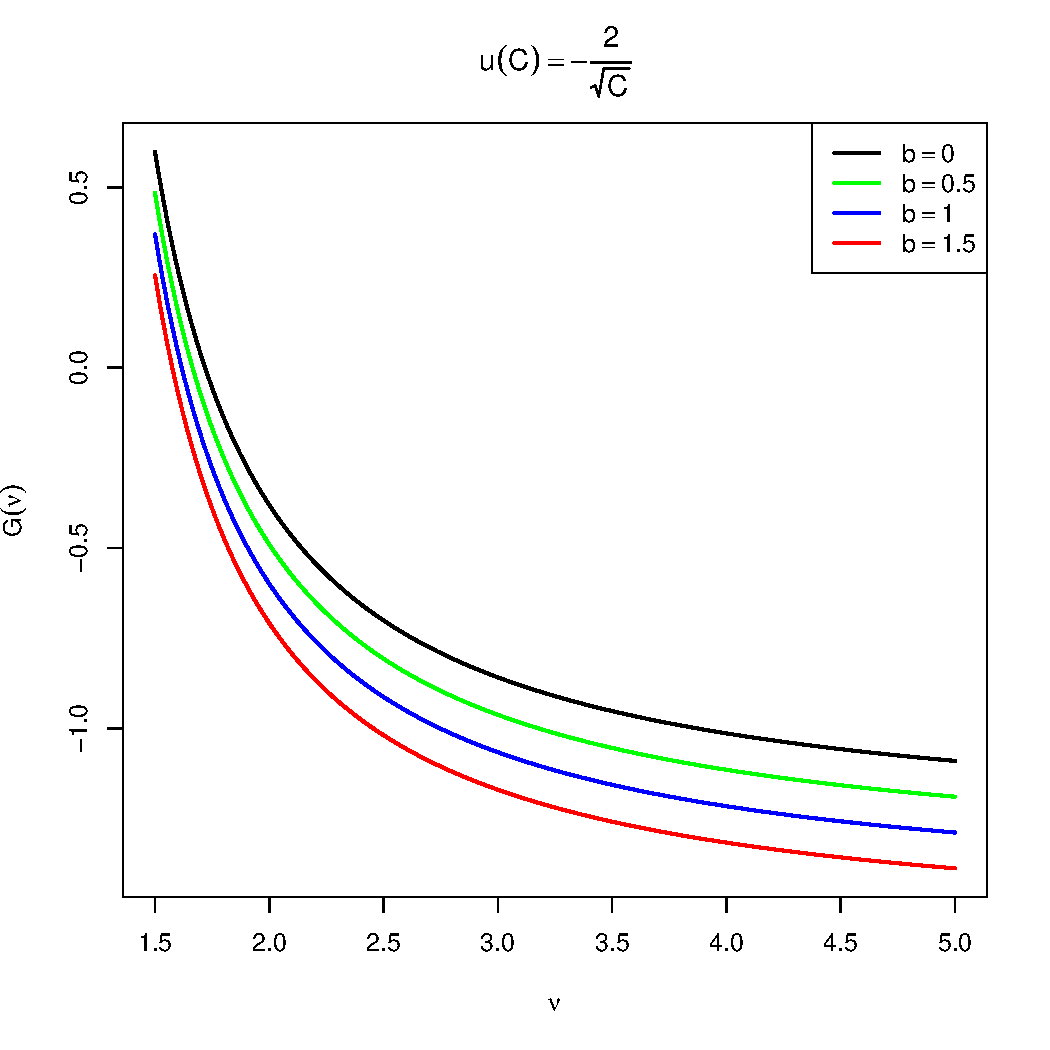
\includegraphics[width=\textwidth]{U_b_t_power.pdf}
  %   \caption{$G(\nu)$ of power-utility function}
  %   \label{fig:U_b_t_power}
  % \end{subfigure}
  \begin{minipage}{0.5\linewidth}
    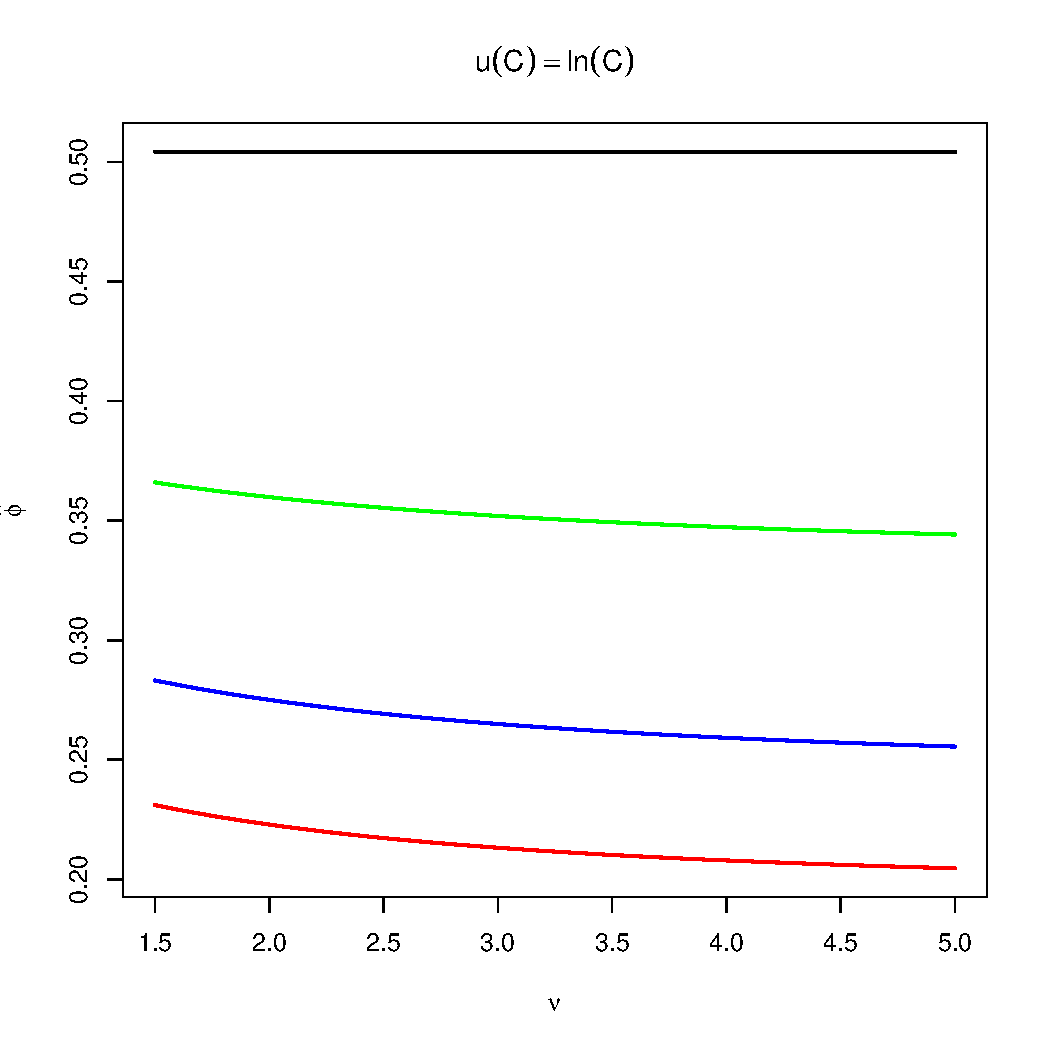
\includegraphics[width=\textwidth]{phi_hat_b_t_log.pdf}
  \end{minipage}\hfill
  \begin{minipage}{0.5\linewidth}
    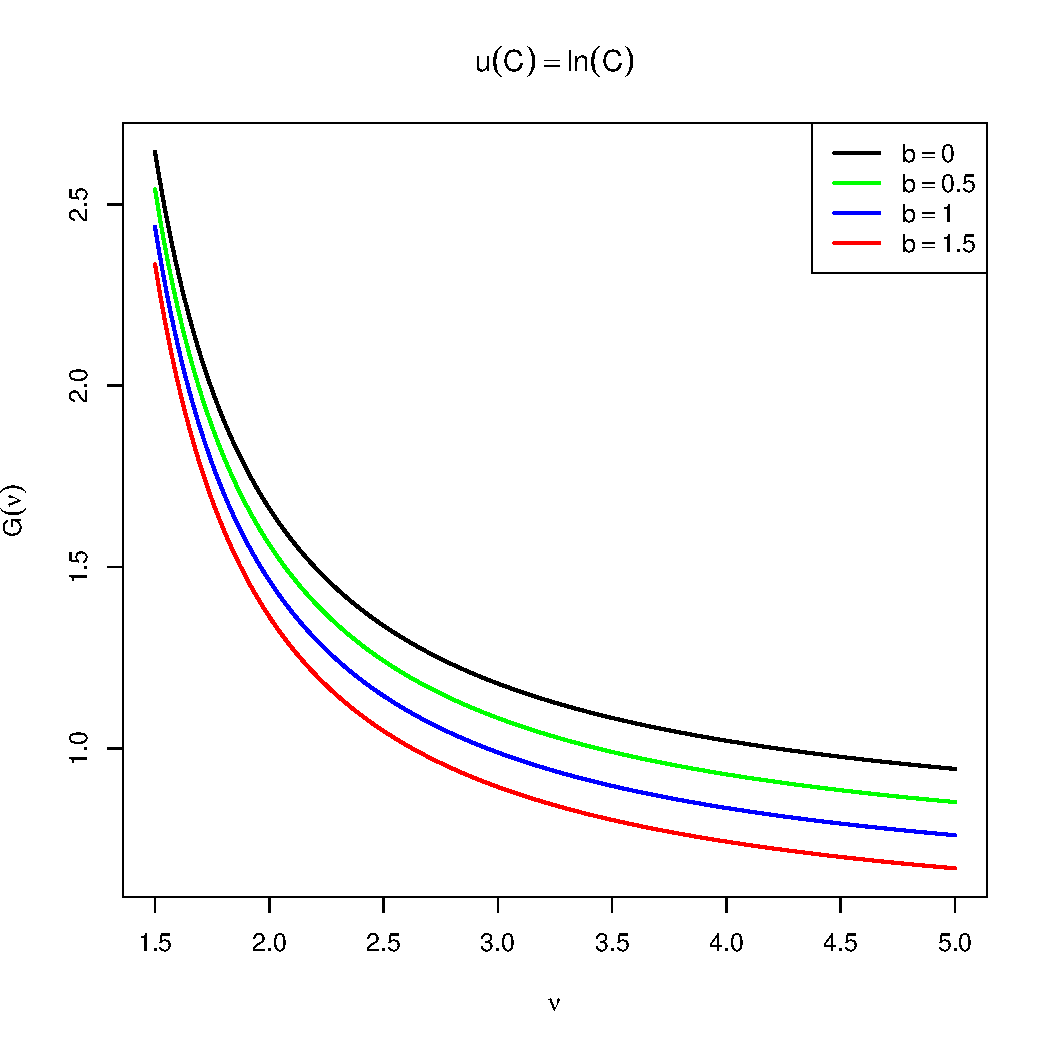
\includegraphics[width=\textwidth]{U_b_t_log.pdf}
  \end{minipage}
  \begin{minipage}{0.5\linewidth}
    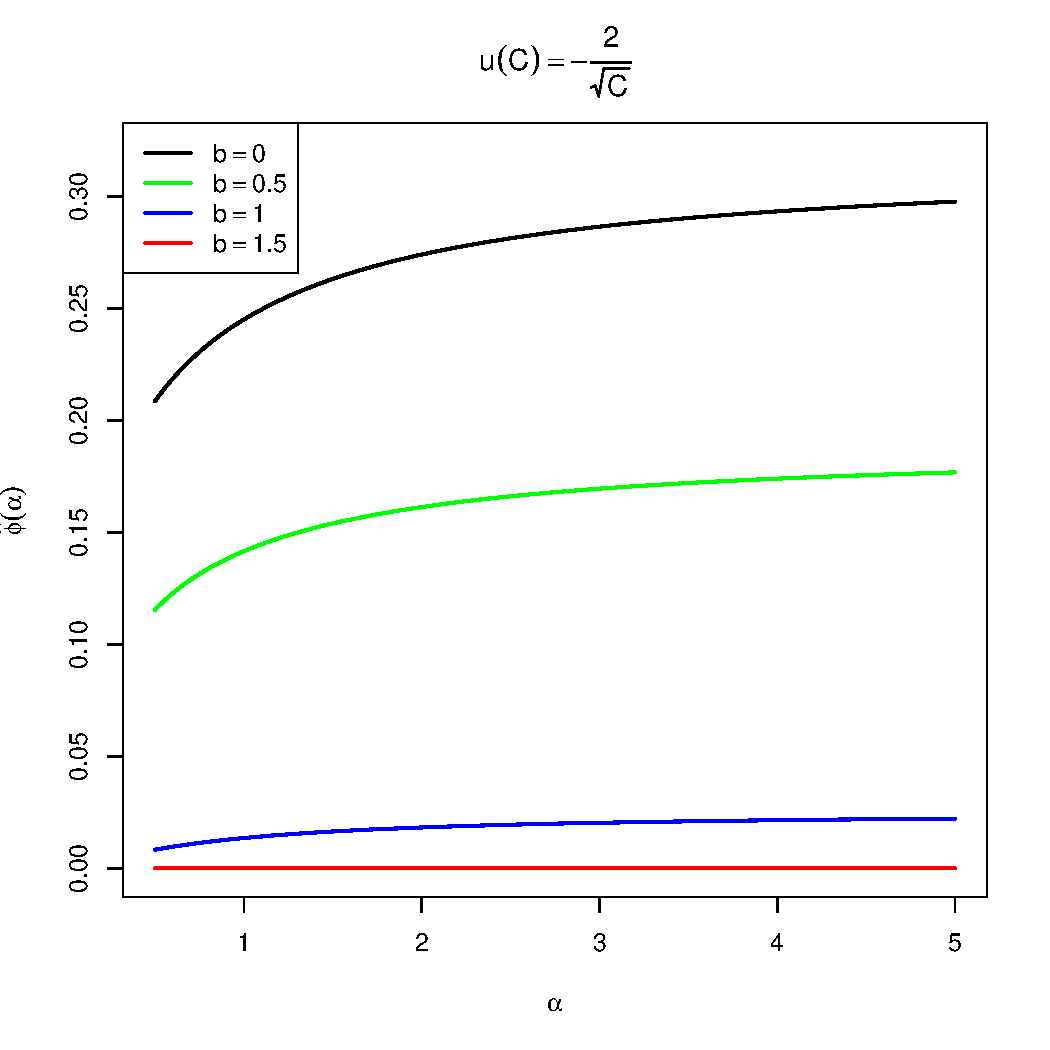
\includegraphics[width=\textwidth]{phi_hat_b_t_power.pdf}
  \end{minipage}\hfill
  \begin{minipage}{0.5\linewidth}
    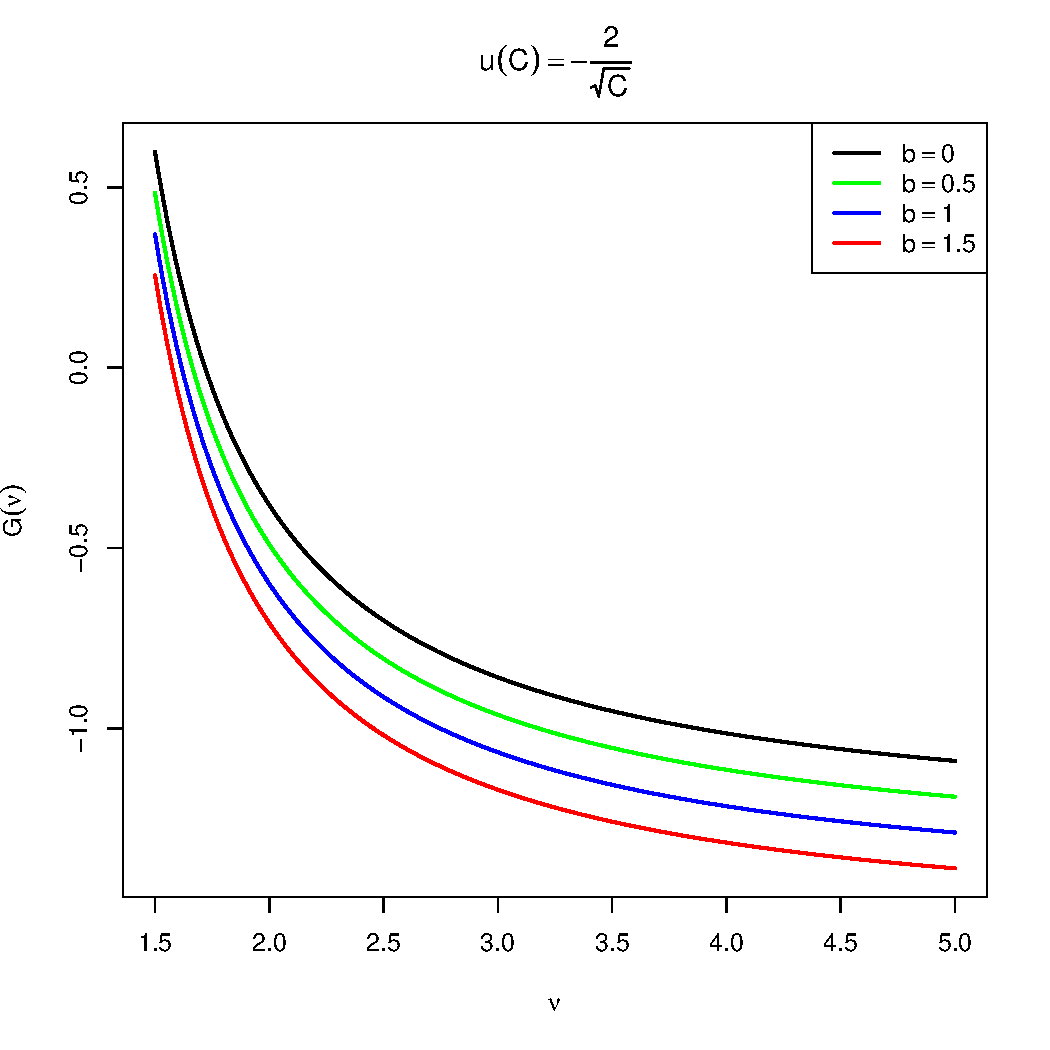
\includegraphics[width=\textwidth]{U_b_t_power.pdf}
  \end{minipage}
  \caption{$\hat\phi$ and $G(\nu)$
    \label{fig:phi_hat_U}
  }
\end{figure}

%% However, this is not necessarily the case when $b > 0$. For example,
%% consider the case when $q = 0$ and $\hat\phi = 1$. This may be
%% viewed an approximation to the situation where the interest rate $r$ is
%% vanishingly low while the investor is more conservative than
%% greedy. In this case we have
%% \begin{eqnarray*}
%%   \mathcal U(F, \phi) = \int_{0}^{\infty} e^{-b x} f(x, \nu) dx
%% \end{eqnarray*}
%% Thus by the 1st case of lemma \ref{lemma:I} and lemma \ref{lemma:II},
%% $\opd{\nu}\mathcal U(F, \phi) > 0$. In this extreme case, the investor
%% would rather seek the largest $\nu$ or in other words, the lightest
%% tail in the market.

\subsubsection{power-utility function}
In this section we consider the case when the utility function
$u(\cdot)$ takes the form
\[
u(C) = -{1 \over \xi} C^{-\xi}
\]
One can see from figure \ref{fig:phi_hat_U_power} that both $\hat
\phi$ and $G(\nu)$ are monotonically decreasing with $\nu$ as in the
case of a log-utility function.
\begin{figure}[htb!]
  \begin{minipage}{0.5\linewidth}
    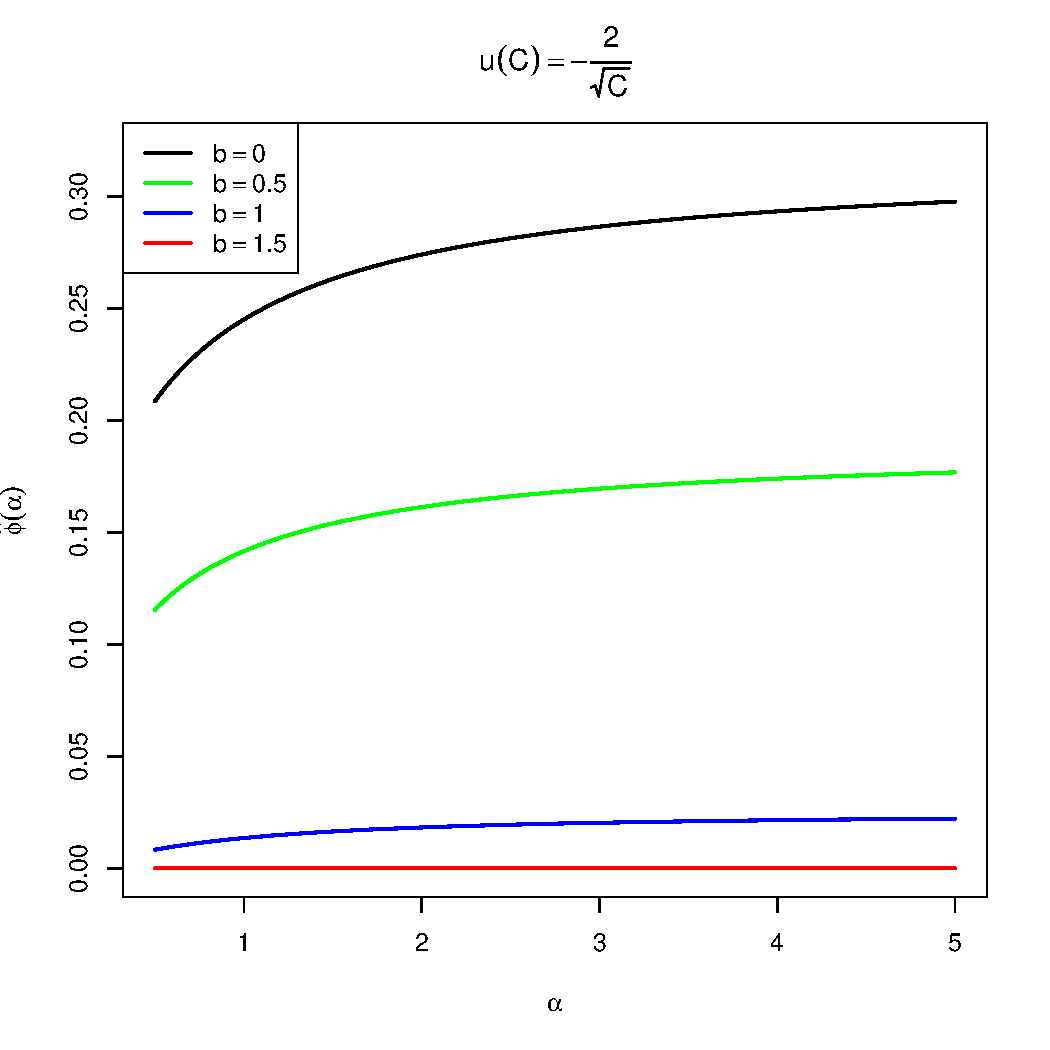
\includegraphics[width=\textwidth]{phi_hat_b_t_power.pdf}
  \end{minipage}\hfill
  \begin{minipage}{0.5\linewidth}
    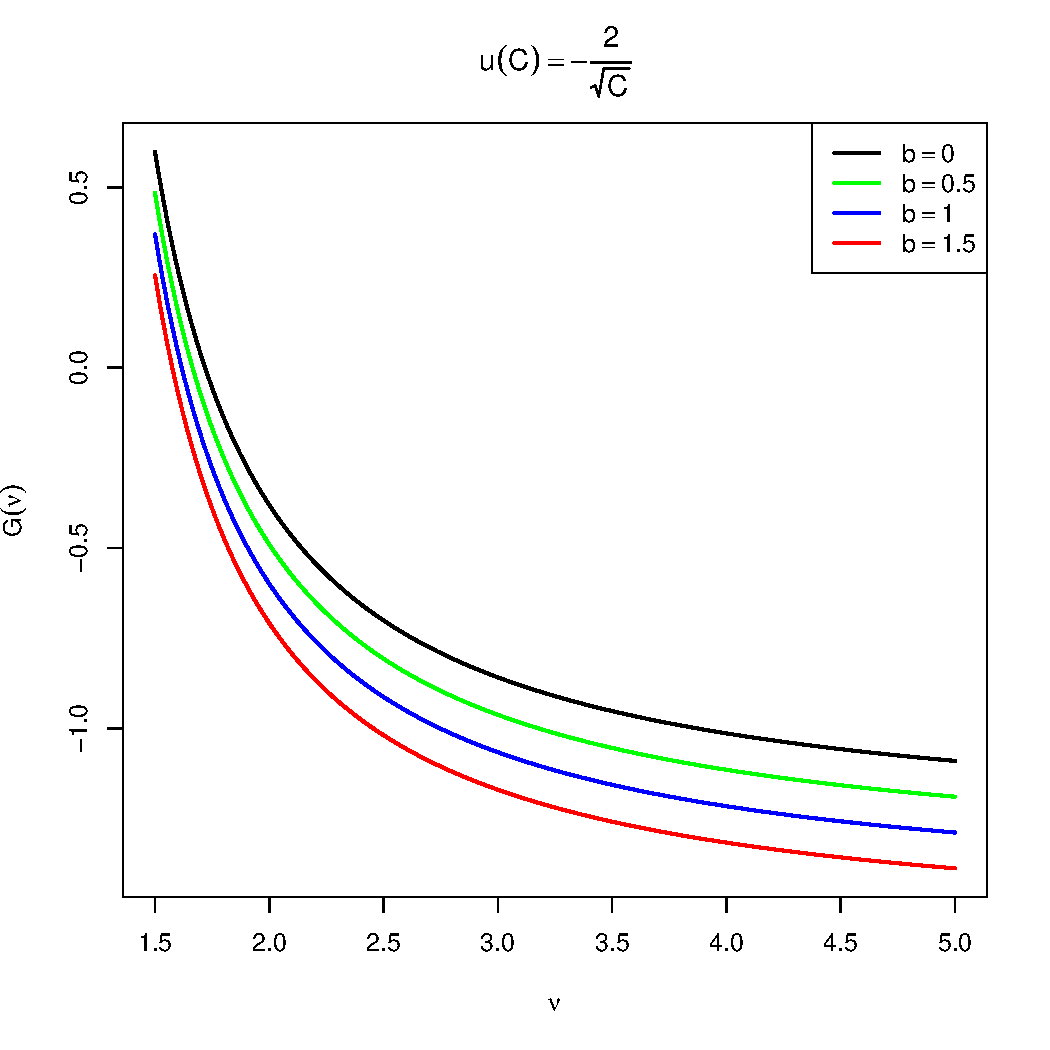
\includegraphics[width=\textwidth]{U_b_t_power.pdf}
  \end{minipage}
  \caption{$\hat\phi$ and $G(\nu)$ when the utility
    function is $u(C) = -{2 \over \sqrt{C}}$
  }
  \label{fig:phi_hat_U_power}
\end{figure}

\section{Conclusion}
\label{sec:4}
TODO: Summarize and conclude that all correlated series share the same
tail index; their tail functions differ from each other via their
scale parameters.

\appendix
\section{Proof of lemma \ref{lemma:I}}
\begin{proof}
  Clearly
  \begin{eqnarray*}
    && {\pd \E h(X) \over \pd \theta} \\
    &=& \int_a^b h(x) {\pd f \over \pd \theta}(x, \theta) dx \\
    &=& \underbrace{\int_a^{x_0} h(x) {\pd f \over \pd \theta}(x, \theta) dx}_{I_1}
    + \underbrace{\int_{x_0}^b h(x) {\pd f \over \pd \theta}(x, \theta) dx}_{I_2}
  \end{eqnarray*}
  \begin{enumerate}
  \item When $h(x)$ is decreasing on $(a, b)$ and ${\pd f \over \pd \theta}(x,
    \theta) > 0$ on $(a, x_0)$
    \[
    I_1 > h(x_0) \int_a^{x_0} {\pd f \over \pd \theta}(x, \theta) dx
    \]
    Similarly, because ${\pd f \over \pd \theta}(x, \theta) < 0$ for $x \in (x_0, b)$ and
    $h(x)$ is decreasing, we have
    \begin{eqnarray*}
      I_2 &=& \int_{x_0}^b -h(x_0)
      \left|{\pd f \over \pd \theta}(x, \theta) \right| dx \\
      &>& -h(x_0)
      \int_{x_0}^b \left| 
        {\pd f \over \pd \theta}(x, \theta)
      \right| dx
    \end{eqnarray*}
    Finally we have
    \begin{eqnarray*}
      {\pd \E h(X) \over \pd \theta}
      > h(x_0) \int_a^b {\pd f \over \pd \theta}(x, \theta) dx
      = h(x_0) {\partial \over \partial \theta} \int_a^b f(x, \theta) dx
      = 0
    \end{eqnarray*}
  \item If $h(\cdot)$ is increasing and $\exists x_0 \in (a, b)$ such that 
    ${\pd f \over \pd \theta}(x_0; \theta) < 0$ on $(a, x_0)$  while
    ${\pd f \over \pd \theta}(x_0; \theta) > 0$ on $(x_0, b)$
    \begin{eqnarray*}
      I_1 &=&
      \int_a^{x_0} -h(x)
      \left| {\pd f \over \pd \theta}(x, \theta) \right| dx \\
      &>&
      -h(x_0) \int_a^{x_0}
      \left| {\pd f \over \pd \theta}(x, \theta) \right| dx
    \end{eqnarray*}
    and obviously
    \[
    I_2 > h(x_0) \int_{x_0}^b
    {\pd f \over \pd \theta}(x, \theta) dx
    \]
    So
    \[
    {\pd \E h(X) \over \pd \theta}
    = I_1 + I_2
    > h(x_0) {\partial \over \partial \theta} \int_a^b f(x, \theta) dx = 0
    \]
  \end{enumerate}
\end{proof}

\section{Proof of lemma \ref{lemma:II}}
\begin{proof}
  Straightforward computation gives
  \begin{eqnarray}
    {\pd f(x, \nu) \over \pd \nu} &=& {
      c(\nu) x^2 (\nu + 1) + (2 \nu x^2 + 2 \nu^2) c'(\nu)
      -
      \nu c(\nu) (x^2 + \nu) \ln(1 + x^2/\nu)
      \over
      2 \nu (x^2 + \nu) (1 + x^2 / \nu)^{\nu/2 + 1/2}
    } \nonumber \\
    &:=& {
      P(x^2, \nu)
      \over
      2 \nu (x^2 + \nu) (1 + x^2 / \nu)^{\nu/2 + 1/2}
    }
    \label{eq:xxie4.1}
  \end{eqnarray}

  While the denominator of the right side of ${\pd f(x, \nu) \over \pd \nu}$ is
  always positive, its nummerator $P(x^2, \nu)$ has a single root:
  \begin{equation}
    \label{eq:xxie5}
    x_0^2 = \nu\exp\left\{
      W\left[
        -\left(1 + {1 \over \nu}\right)
        e^{-1 - 2 c'(\nu)/c(\nu) - 1/\nu}
      \right]
      + 1 + {1 \over \nu} + {2 c'(\nu) \over c(\nu)}
    \right\} - \nu
  \end{equation}
  where $W(\cdot)$ is the principle branch of the Lambert $W$
  function. and $c'(\cdot)$ is the derivative of $c(\cdot)$. To check
  the right side of \eqref{eq:xxie5} for positivity, we first note
  $c'(\nu) > 0$:
  \[
  c'(\nu) = {
    \pi \Gamma(\nu/2 + 1/2) \left\{
      \nu \left[ \Psi(\nu/2 + 1/2) - \Psi(\nu/2)\right] - 1
    \right\}
    \over
    2 \Gamma(\nu/2) (\pi \nu)^{3/2}
  }
  \]
  where $\Psi(\cdot)$ is the digamma function:
  \[
  \Psi(x) = {d \ln[\Gamma(x)] \over d x}
  \]
  \begin{minipage}{0.48\textwidth}
    $\Psi(x)$ \linebreak
    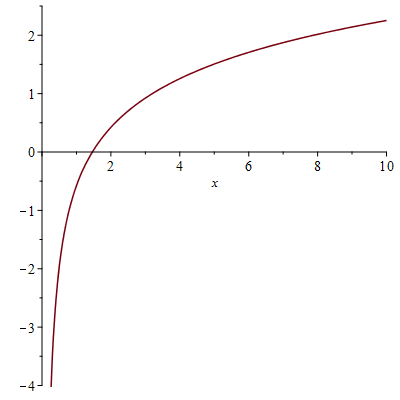
\includegraphics[width=\textwidth]{digamma.png}
  \end{minipage}\hfill
  \begin{minipage}{0.5\textwidth}
    As shown in the figure to the left, $\Psi(x)$ is increasing
    for $x > 0$. Therefore $\Psi(\nu/2 + 1/2) - \Psi(\nu/2) > 0$.
    So we have
    \begin{eqnarray*}
      && \nu \left[
        \Psi(\nu/2 + 1/2) - \Psi(\nu/2)
      \right] - 1 \\
      &\geq& 1 \times \left[
        \Psi(1/2 + 1/2) - \Psi(1/2)
      \right] - 1 \\
      &=& \ln(4) - \ln(e) \\
      &>& 0
    \end{eqnarray*}
    Thus $c'(\nu) > 0$. Furthermore, we recall
    $W(\cdot)$ is increasing on its principle branch. So
  \end{minipage}
  \begin{eqnarray*}
    &&
    W\left[
      -\left( 1 + {1 \over \nu} \right)
      e^{-1 - 2 c'(\nu)/c(\nu) - 1/\nu}
    \right]
    + 1 + {1 \over \nu} + {2 c'(\nu) \over c(\nu)} \\
    &>& 
    W\left[
      -\left( 1 + {1 \over \nu} + {2 c'(\nu) \over c(\nu)} \right)
      e^{-1 - 2 c'(\nu)/c(\nu) - 1/\nu}
    \right]
    + 1 + {1 \over \nu} + {2 c'(\nu) \over c(\nu)} \\
    &=& W(-y e^{-y}) + y
  \end{eqnarray*}
  where
  \[
  y = 1 + {1 \over \nu} + {2 c'(\nu) \over c(\nu)} > 1
  \]
  Now notice
  \[
  \ln(y e^{-y}) = \ln(y) - y
  \]
  is a decreasing function for $y > 1$. Thus $-y e^{-y}$ is an
  increasing function. Hence we have
  \begin{eqnarray*}
    W(-y e^{-y}) + y &>& W(-e^{-1}) + 1 = 0
  \end{eqnarray*}
  Now it is clear
  \[
  \nu\exp\left\{
    W\left[
      -\left(1 + {1 \over \nu}\right)
      e^{-1 - 2 c'(\nu)/c(\nu) - 1/\nu}
    \right]
    + 1 + {1 \over \nu} + {2 c'(\nu) \over c(\nu)}
  \right\} - \nu > 0
  \]
  Now that we have established that ${\pd f \over \pd \nu}(x, \nu) = 0$ has a
  single positive root, it remains to determine the sign of
  ${\pd f \over \pd \nu}(x, \nu)$ on the two sides of the root. For this purpose
  we observe
  \begin{equation}
    \label{eq:xxie5.1}
    P(0, \nu) = 2 \nu^2 c'(\nu) > 0
  \end{equation}
  So we want to investigate ${\pd P \over \pd x}(x, \nu)$:
  \begin{eqnarray}
    {\pd P \over \pd x}(x, \nu) &=&
    2 \nu c'(\nu) + c(\nu) - \nu c(\nu) \ln\left(
      1 + {x \over \nu}
    \right)
    \label{eq:xxie6}
  \end{eqnarray}
  Clearly, $\frac{\pd P}{\pd x}(0, \nu) > 0$. Hence from
  \eqref{eq:xxie5.1} and
  \eqref{eq:xxie6} it is clear
  \begin{equation*}
    \text{sign}\left[
      \pd{f}{\nu}(x, \nu)
    \right]
    = \left\{
    \begin{array}{rl}
      1 & 0 < x < x_0 \\
      -1 & x > x_0
    \end{array}
    \right.
  \end{equation*}
  where $x_0$ is the positive root of \eqref{eq:xxie5}.
\end{proof}

\section{Proof of Theorem \ref{thrm:I}}
\label{sec:thrmI_proof}
\begin{proof}
  Let
  \begin{equation}
    \label{eq:xxie2}
    \hat \phi := \text{argmax}_{0 < \phi \leq 1} \mathcal U(F, \phi)
  \end{equation}
  We have
  \[
  G(F) = \mathcal U(F, \hat\phi)
  \]
  It follows
  \begin{eqnarray}
    \pd{G(F)}{\alpha}
    &=&
    \pd{\mathcal U(F, \phi)}{\alpha}(\alpha, K, \hat\phi)
    + \pd{\mathcal U(F, \phi)}{\phi}(\alpha, K, \hat\phi)
    \pd{\hat\phi}{\alpha}(\alpha, K)
    \label{eq:xxie3}
  \end{eqnarray}
  The definition \eqref{eq:xxie2} implies $\forall \alpha > 1$
  \begin{equation}
    \label{eq:xxie4}
    \pd{\mathcal U(F, \phi)}{\phi}(\alpha, K, \hat \phi) = 0
  \end{equation}
  So the second term of \eqref{eq:xxie3} vanishes. It remains to show
  \begin{eqnarray*}
    \pd{\mathcal U(F, \phi)}{\alpha}(\alpha, K, \hat \phi)
    &>& 0
  \end{eqnarray*}
  From \eqref{eq:xxie1.0}, it follows
  \begin{eqnarray*}
    \pd{\mathcal U(F, \phi)}{\alpha}(\alpha, K, \hat\phi)
    = {\partial \over \partial \alpha}\E[u((1 - \hat\phi) e^r + \hat\phi e^X) \1{X < 0}]
  \end{eqnarray*}
  The function $u((1 - \hat\phi) e^r + \hat\phi e^X)$ is obviously
  increasing with $X$. It follows
  \begin{eqnarray*}
    && \pd{f(x; \alpha, K)}{\alpha} \\
    &=& {\partial \over \partial \alpha} {\alpha K^\alpha \over (K - x)^{\alpha + 1}} \\
    &=&
    - {K^\alpha \over (K - x)^{\alpha + 1}}
    \left[
      \alpha
      \ln\left(
        1 - {x \over K}
      \right) - 1
    \right]
  \end{eqnarray*}
  It is easily checked that when $x < K(1 - e^{1/\alpha}) < 0$,
  \[
  {\partial \over \partial \alpha} {\alpha K^\alpha \over (K - x)^{\alpha + 1}} < 0
  \]
  and when $K(1 - e^{1/\alpha}) < x < 0$,
  \[
  {\partial \over \partial \alpha} {\alpha K^\alpha \over (K - x)^{\alpha + 1}} > 0
  \]
  This is the second case of lemma \ref{lemma:I}. So we have
  \begin{eqnarray*}
    \pd{\mathcal U(F, \phi)}{\alpha}(\alpha, K, \hat\phi) &>& 0
  \end{eqnarray*}
  As for $\pd{G(F)}{K}$, by the same argument as for
  $\pd{G(F)}{\alpha}$, it suffices to show
  \[
  \pd{\mathcal U(F, \phi)}{K}(\alpha, K, \hat\phi) < 0
  \]
  We have
  \[
  \pd{\mathcal U(F, \phi)}{K}(\alpha, K, \hat\phi)
  = {\partial \over \partial K} \E \left[
    u((1 - \hat\phi) e^r + \hat\phi e^X) \1{X < 0}
  \right] 
  \]
  and
  \begin{eqnarray*}
    && \pd{f(x; \alpha, K)}{K} \\
    &=& {\partial \over \partial K} {\alpha K^\alpha \over (K - x)^{\alpha + 1}} \\
    &=&
    -\alpha K^{\alpha - 1} {
      \alpha x + K
      \over
      (K - x)^{\alpha + 2}
    }
  \end{eqnarray*}
  Clearly, when $x < -\alpha/K$
  \[
  {\partial \over \partial K} {\alpha K^\alpha \over (K - x)^{\alpha + 1}} > 0
  \]
  and when $-\alpha/K < x < 0$
  \[
  {\partial \over \partial K} {\alpha K^\alpha \over (K - x)^{\alpha + 1}} < 0
  \]
  So by the 1st case of remark \ref{remark:I} we conclude
  \[
  \pd{\mathcal U(F, \phi)}{K}(\alpha, K, \hat\phi) < 0  
  \]
\end{proof}

\bibliographystyle{unsrt}
\bibliography{../../thesis/econophysics}
\end{document}
